\documentclass[conference]{IEEEtran}

\usepackage[utf8]{inputenc}
\usepackage[T1]{fontenc}
\usepackage{cite}
\usepackage{array}
\usepackage{tabularx}
\usepackage{booktabs}
\usepackage{enumitem}
\usepackage{microtype}
\usepackage{cuted}
\usepackage{amsmath,amssymb}
\usepackage{float}
\usepackage{graphicx}
\usepackage{xcolor}
\usepackage{url}

\newcolumntype{Y}{>{\raggedright\arraybackslash}X}
\newcolumntype{P}[1]{>{\raggedright\arraybackslash}p{#1}}

\begin{document}

\title{Empirical Evaluation of Greedy t-Spanners: The Impact of Graph Topology on Path Stretch and Edge Sparsity}

\author{
\IEEEauthorblockN{Abdullah Mohammed Khalid Hashim, Sultan Almuhammadi}
\IEEEauthorblockA{
\textit{College of Computer Science \& Engineering}\\
\textit{King Fahd University of Petroleum \& Minerals}\\
Dhahran, Saudi Arabia
}
}

\maketitle
\raggedbottom
\setlength{\textfloatsep}{10pt plus 2pt minus 2pt}

\begin{abstract}
Graph spanners reduce network complexity while preserving bounded shortest-path distances, yet the empirical performance of the classical greedy $t$-spanner across non-geometric network topologies remains insufficiently characterized. This study investigates how graph topology influences edge sparsity and path distortion through $3,600$ spanner constructions across $120$ independent unweighted graphs ($N=1,000$, $\bar{d}\approx3.79\text{--}4.04$). Four canonical topologies were evaluated: Barab\'{a}si--Albert (BA), Watts--Strogatz (WS), Erd\H{o}s--R\'{e}nyi (ER), and perturbed 2D grids (GRID), under stretch factors $t\in\{3,5,7\}$. Each graph underwent $10$ randomized edge permutations per stretch factor, with path distortion measured using $1,000$ sampled vertex pairs and graph-level statistical aggregation. Results reveal substantial topology-dependent differences: WS networks prune $34.1\%$ of edges at $t=3$ and $40.4\%$ at $t=7$, whereas ER networks prune only $2.0\%$ and $24.6\%$ (retaining $98.0\%$ and $75.4\%$, respectively). At $t=7$, BA exhibits significantly higher multiplicative stretch than GRID ($1.602$ versus $1.210$, $p<10^{-10}$), contrary to the hypothesized advantage of scale-free hubs. However, BA incurs lower mean additive delay ($+2.22$ versus $+3.64$ hops), revealing a baseline path-length dilution effect. Structural analysis further identifies strong associations between hub prominence and tail stretch ($r=0.91$). While configuration-level mean stretch ($\bar{s}\le1.602$) and sampled maximum stretch over random vertex pairs remain substantially below $t$ (mean sampled slack of $2.34$ units at $t=7$), exact edge-level verification confirms that global worst-case stretch attains $t$ in all $3,600$ constructions. These findings demonstrate that graph topology substantially influences greedy-spanner performance and highlight the importance of evaluating both multiplicative stretch and additive hop delay when assessing sparsification trade-offs.
\end{abstract}

\begin{IEEEkeywords}
Graph Spanners, Greedy Algorithm, Graph Topology, Path Stretch, Edge Sparsity
\end{IEEEkeywords}



% ============================================================================
% SECTION I: INTRODUCTION
% ============================================================================
\section{Introduction}

Dense graphs appear naturally in many computational domains such as communication backbone, peer-to-peer overlays, and social networks. Performing shortest path queries, routing algorithms, or state synchronization on a dense graph can be computationally and memory intensive \cite{ref1}. Graph sparsification addresses this problem by finding a sparse subgraph which retains important properties of the original graph \cite{ref1}. In particular, a multiplicative $t$-spanner reduces edge count while guaranteeing that shortest-path distances between all vertex pairs expand by at most a factor of $t$ \cite{ref2, ref3, ref4}.

Although the standard greedy $t$-spanner algorithm \cite{ref2} is proven to be existentially optimal across broad graph classes \cite{ref5}, recent theoretical and practical studies demonstrate that worst-case existential optimality does not guarantee uniform performance across individual network topologies \cite{ref6, ref7}. Existing empirical evaluations have largely focused on geometric Euclidean spanners \cite{ref8, ref9, ref7}, multi-level additive spanners \cite{ref10}, decoupled weighted instances \cite{ref6}, or cycle-free tree $t$-spanners \cite{ref11, ref12}. Consequently, the topology-dependent stretch--sparsity trade-off of the standard greedy $t$-spanner on unweighted graphs remains insufficiently characterized under controlled network size and baseline density.

This study presents a controlled empirical evaluation isolating the impact of four canonical topologies, scale-free (Barab\'{a}si--Albert) \cite{ref13}, small-world (Watts--Strogatz) \cite{ref14}, uniform random (Erd\H{o}s--R\'{e}nyi) \cite{ref15}, and planar 2D grids, on unweighted greedy $t$-spanners ($t \in \{3, 5, 7\}$) under matched network size ($N = 1,000$) and approximately matched average degree ($\bar{d} \approx 3.8\text{--}4.0$).

The primary contributions of this paper are:

\begin{itemize}
    \item A controlled experimental evaluation of $3,600$ spanner constructions across $120$ independent baseline networks, employing static node-pair sampling and nested instance-level aggregation to ensure statistical rigor.

    \item Empirical evidence linking local clustering to early edge pruning at $t=3$, and identifying elevated 95th-percentile tail stretch in scale-free networks at $t=7$.

    \item A comparative analysis of scale-free networks and planar grids, highlighting the distinction between multiplicative stretch ratios and absolute additive hop delays.
\end{itemize}

The remainder of this paper is organized as follows. Section~II defines the graph-theoretic preliminaries of $t$-spanners and the four canonical topologies. Section~III reviews related literature and establishes the research gap. Section~IV formalizes the research questions and hypotheses. Section~V details the experimental methodology and statistical design. Section~VI presents and discusses the empirical results and practical guidelines. Section~VII addresses threats to validity, and Section~VIII concludes the paper with directions for future work.

% ============================================================================
% SECTION II: BACKGROUND
% ============================================================================

\section{Background}

\subsection{Multiplicative $t$-Spanners and Greedy Construction}

Let $G = (V, E_G)$ be a connected, undirected, unweighted graph, where $d_G(u,v)$ denotes the shortest-path distance (in hops) between vertices $u$ and $v$.

A subgraph $H = (V, E_H)$, where $E_H \subseteq E_G$, is a multiplicative $t$-spanner ($t \geq 1$) if:

\begin{equation}
    d_H(u,v) \leq t \cdot d_G(u,v),
    \quad \forall u,v \in V.
\end{equation}

This guarantees that shortest-path distances increase by at most a factor of $t$ \cite{ref2, ref3}. By the triangle inequality, this global condition is satisfied if and only if every original edge $(u,v) \in E_G$ satisfies $d_H(u,v) \leq t$ \cite{ref2}.

The standard greedy algorithm \cite{ref5, ref2} constructs a spanner by initially setting $H = (V, \emptyset)$ and processing the original edges sequentially. For unweighted graphs, where all edge weights equal $1$, the edges may be processed in a random permutation to control ordering effects.

For each candidate edge $(u,v)$, the algorithm applies the following rule:

\begin{equation}
    (u,v) \text{ is added to } E_H
    \iff d_H(u,v) > t.
\end{equation}

Otherwise, the edge is discarded as redundant \cite{ref16, ref2}.

Unlike tree $t$-spanners \cite{ref11, ref12}, which prohibit all cycles, the general greedy $t$-spanner may retain longer cycles while excluding cycles of length at most $t+1$ (for integer $t \ge 1$). Consequently, its girth is at least $t+2$ whenever cycles exist, and graph connectivity is preserved \cite{ref2, ref17, ref4}.


\subsection{Benchmark Network Topologies}
To isolate structural effects, researchers model distinct topological properties using synthetic generators:
\begin{itemize}
    \item \textit{Barab\'{a}si--Albert (BA) \cite{ref13}:} Represents scale-free networks via preferential attachment, yielding power-law degree distributions with prominent hubs and short global paths.
    \item \textit{Watts--Strogatz (WS) \cite{ref14}:} Represents small-world networks by rewiring a ring lattice, combining high local clustering (triadic closure) with short path lengths.
    \item \textit{Erd\H{o}s--R\'{e}nyi (ER) \cite{ref15}:} Represents uniform random graphs where independent edge placement yields an approximately Poisson degree distribution (prior to connectivity repair) and near-zero clustering.
    \item \textit{2D Planar Grids (GRID):} Represents rigid spatial lattices characterized by bounded degree ($\Delta \le 4$), zero triangles (bipartite girth of $4$), and long shortest paths.
\end{itemize}


% ============================================================================
% SECTION III: LITERATURE REVIEW
% ============================================================================
\section{Literature Review}

\subsection{Theoretical Baselines and the Instance-Optimality Anomaly}
The standard greedy algorithm is one of the most studied approaches for constructing sparse and light-weight graph spanners \cite{ref4}. Mathematically, the greedy spanner is proven to be existentially optimal (or near optimal) regarding both size and weight parameters for several important graph families \cite{ref5}. Existential optimality means that the worst-case performance of the greedy spanner over a particular graph family is asymptotically comparable to the worst-case performance of optimal spanners over that family \cite{ref5}. Building on this foundation, Le and Solomon \cite{ref18} developed a unified meta-framework that transforms sparse spanner constructions into near-optimal light spanners across general and minor-free graph classes, while Bodwin \cite{ref17} established an alternate direct proof of greedy spanner lightness by extending classical Moore-bound girth arguments. Concurrently, Bodwin and Flics \cite{ref19} established conditional lower bounds on the lightness of spanners in general weighted graphs under the Erd\H{o}s girth conjecture.

However, recent theoretical and experimental studies have challenged the assumption that this theoretical optimality translates uniformly across all graph structures. Le et al.\ demonstrated that the greedy spanner is far from instance-optimal by designing explicit ``hard instances'' of point sets in the Euclidean plane \cite{ref7}. On these specific hard instances, the greedy $(1 + x\epsilon)$-spanner produces $\Omega_x(\epsilon^{-1/2})$ times the number of edges and $\Omega_x(\epsilon^{-1})$ times the weight compared to the optimally sparsest and lightest $(1+\epsilon)$-spanners, respectively \cite{ref7}. This divergence demonstrates that worst-case theoretical optimality does not necessarily guarantee comparable performance on individual graph instances \cite{ref7}.

This structural vulnerability is further supported by B\"{o}kler et al., who evaluated standard and augmented greedy algorithms on decoupled $\alpha$-spanner instances, where weights and lengths are independent \cite{ref6}. Their experiments found that $95.8\%$ of practical real-world instances could be solved exactly for $\alpha \le 3$, typically using a path-based integer linear programming approach \cite{ref6}. Although traditional greedy algorithms often produced high-quality solutions with low running times, the researchers also discovered specific practical topology instances, such as SBM (Stochastic Block Model) arising in graph drawing, where the standard greedy algorithm systematically attains solutions of ``abysmal quality'' \cite{ref6}.

\subsection{Empirical Measurements of Stretch and Sparsity in Practice}
To understand the practical utility of sparsifiers, researchers often compare their empirical performance against average stretch and edge reduction. Chen et al.\ developed a framework with $12$ sparsification algorithms, including $t$-spanners, against $16$ graph metrics to evaluate the algorithms using $14$ real-world graphs \cite{ref1}. They found that $t$-spanners successfully preserve graph connectivity, though no single sparsifier performs best across all properties \cite{ref1}.

Their experiments also demonstrated that increasing the pruning rate generally reduces the ability of sparsification algorithms to preserve graph properties \cite{ref1}. Some sparsifiers exhibit an ``elbow point,'' beyond which performance declines sharply because the remaining edges are insufficient to preserve particular properties \cite{ref1}. For example, the Local Degree sparsifier experienced a sudden decline in performance when the pruning rate increased from $0.8$ to $0.9$, as the remaining edges could no longer maintain graph connectivity \cite{ref1}. However, unlike such sparsifiers, $t$-spanners preserve the connectivity of the original graph and provide a theoretical bound on shortest-path expansion \cite{ref1, ref4}. In a closely related empirical study, K\={o}shima et al.\ evaluated density--accuracy trade-offs of graph spanners on real-world social and information networks, showing that ultra-sparse tree-like decompositions often incur suboptimal additive distance error whereas retaining slightly higher edge density substantially improves distance estimation accuracy \cite{ref20}.

When algorithms are compared on standard datasets, the greedy approach consistently produced high-quality metrics. Chimani and Stutzenstein showed that the basic greedy algorithm (ADDJS) generally generates highly sparse and light spanners in practice within reasonable computation times, outperforming complex approximation alternatives like BBMRY by a large margin across the Random, Steinlib, and TSPLIB benchmark suites \cite{ref21}. The alternative approximation algorithms generally required substantially longer computation times while producing less competitive spanner quality \cite{ref21}. This was supported by the comprehensive study by Farshi and Gudmundsson of geometric Euclidean $t$-spanners that showed that the greedy graph provides a surprisingly high level of quality in terms of the number of edges, weight, maximum degree and number of crossings \cite{ref8, ref9}. They also discovered, however, a fundamental geometric anomaly; the greedy graph exhibits a larger geometric spanner diameter than several alternative constructions \cite{ref9}.

Because exact greedy construction incurs a severe shortest-path verification bottleneck on large networks, recent algorithmic engineering has focused on scalable approximations. In two-dimensional geometric settings, Ghosh \cite{ref22} proposed the parallel $\Theta$-Greedy algorithm to construct spanner ``doppelg\"{a}ngers'' that empirically match the average degree and lightness of exact greedy spanners at low stretch factors while achieving near-quadratic practical scaling. For unweighted general graphs, Haeupler et al.\ \cite{ref23} demonstrated that sequential greedy construction can be parallelized by iteratively adding matchings of $t$-unspanned edges, with sparsity guarantees established via length-constrained expander decompositions, though relaxing sequential edge inspection permits cycles of length $4$ to remain in the spanner regardless of $t$.

In communication network applications, the trade-off between the cost of the network and path delay is also important. Network simulation can be used to evaluate algorithms and protocols under controlled conditions \cite{ref24}, while compact routing research has demonstrated the trade-off between routing storage requirements and path stretch \cite{ref25}. These applications show the need to maintain the shortest paths while minimizing the network complexity.

Farley et al.\ \cite{ref16} analyzed the trade-off between network cost and latency through simulations of greedy $t$-spanners (denoted as $k$-spanners in their paper) on purely random and Waxman locality-preference network topologies, addressing both broadcast and multicast message delivery. Their work shows that by changing the stretch parameter $k$, the spanner can trade off between minimizing network costs and increasing path delays. Their simulations showed that greedy spanners provide significant edge reduction: for graphs with an average degree of $8$, a $4$-spanner retained approximately $30\%$ of the original edges under length- and weight-based distance measures, whereas hop-based spanners retained approximately $46\text{--}52\%$ of the original edges \cite{ref16}. However, this edge reduction increased the ratio of average hop distances to approximately $1.4$, which remained substantially lower than that of minimum-distance spanning trees. They also observed that spanners could exhibit larger hop diameters than spanning trees under certain stretch settings, highlighting that improvements in mean path ratios do not necessarily imply improvements in every distance-related metric \cite{ref16}.

\subsection{Topology-Specific Studies and the Tree Spanner Limitation}
Couto et al.\ investigated topological effects by evaluating the $t$-admissibility problem: finding a subgraph where the distance between adjacent vertices is at most $t$ \cite{ref12}. To evaluate their heuristic algorithms, they performed experiments with various distinct random topologies: Barab\'{a}si--Albert graphs (scale-free), Erd\H{o}s--R\'{e}nyi graphs, Watts--Strogatz graphs, and Bipartite graphs \cite{ref12}. Cunha et al.\ advanced this approach by adding nine new heuristics based on vertex importance across the exact same topologies (Barab\'{a}si--Albert, Erd\H{o}s--R\'{e}nyi, Watts--Strogatz, and bipartite) to obtain the exact stretch indexes \cite{ref11}.

Related research has also examined alternative spanner formulations, including empirical evaluations of multi-level weighted additive spanners \cite{ref10} and theoretical lightness bounds for edge fault-tolerant spanners \cite{ref26}. Ahmed et al.\ investigated multi-level weighted additive spanners, evaluating several algorithms in terms of running time and sparsity using graphs generated through Erd\H{o}s--R\'{e}nyi, Watts--Strogatz, Barab\'{a}si--Albert, and random geometric models \cite{ref10}. Their experiments evaluated the practical sparsity, running time, and approximation quality of multi-level weighted additive spanner constructions \cite{ref10}. They also developed an approach based on modifying an initialization parameter that improved the quality of practical spanners at the expense of a small increase in running time \cite{ref10}. However, their research focused on multi-level weighted additive spanners with subsetwise distance requirements rather than general greedy multiplicative $t$-spanners \cite{ref10}. Therefore, although this study demonstrates the usefulness of evaluating spanner algorithms across distinct network structures, it does not directly establish how those structures influence the average multiplicative stretch and edge sparsity of the standard greedy $t$-spanner.

However, a major limitation exists within the topological evaluations conducted by Couto et al.\ and Cunha et al.: both studies restricted their research entirely to generating tree $t$-spanners \cite{ref11, ref12}. Tree spanners are heavily constrained subgraphs that forbid any cycles, completely differentiating them from general $t$-spanners \cite{ref11, ref12}. More specifically, a tree $t$-spanner must be a spanning tree in which the distance between any two adjacent vertices in the original graph is at most $t$ in the generated tree \cite{ref11}.

The computational characteristics of this problem further distinguish it from general spanner construction. The $t$-admissibility decision problem is polynomial-time solvable for $t \le 2$, NP-complete for $t \ge 4$, and remains an open problem for $t = 3$ \cite{ref11}. Consequently, the structural restrictions and computational requirements of tree-spanner algorithms differ significantly from those of unconstrained greedy $t$-spanners.

\subsection{Synthesis and Research Gap}
Current research establishes a clear separation. While general greedy $t$-spanners are existentially optimal \cite{ref5} and admit near-optimal lightness bounds \cite{ref17, ref18}, their performance degrades to ``abysmal quality'' on specific structural instances \cite{ref6, ref7}. Furthermore, although researchers recognize the importance of testing algorithms on different network structures, including both scale-free (Barab\'{a}si--Albert) and small-world (Watts--Strogatz) models, existing evaluations address different spanner formulations. These include tree spanners \cite{ref11, ref12}, multi-level weighted additive spanners \cite{ref10}, geometric Euclidean spanners \cite{ref8, ref9, ref7, ref22}, parallel unweighted matchings \cite{ref23}, fault-tolerant spanners \cite{ref26}, real-world density--accuracy evaluations \cite{ref20}, and decoupled multiplicative spanners \cite{ref6}.

Thus, there remains an unaddressed gap in the reviewed research concerning the controlled empirical evaluation of general (non-geometric) graph topologies, specifically comparing scale-free hubs against rigid local grids and others, on the average stretch and edge sparsity of standard greedy $t$-spanners. A systematic evaluation of these structural classes is needed to determine whether specific topological properties mitigate or contribute to the performance anomalies identified in previous research.


\section{Research Questions and Hypotheses}

To operationalize the study's objective, we evaluate three central research questions and their corresponding null ($H_0$) and alternative ($H_a$) hypotheses:

\subsection{RQ1 (Topological Effect)}
Does network topology significantly affect the edge retention ratio and empirical path stretch of unweighted greedy $t$-spanners?

\noindent
\textit{$H_{0,1}$ (Null):}
Mean edge retention and empirical stretch do not differ significantly across Barab\'{a}si--Albert, Watts--Strogatz, Erd\H{o}s--R\'{e}nyi, and 2D grid topologies.

\noindent
\textit{$H_{a,1}$ (Alternative):}
At least one network topology exhibits a statistically significant difference in mean edge retention or empirical path stretch.

\subsection{RQ2 (Hubs vs.\ Grids)}
Does the presence of structural hubs in scale-free networks protect paths from severe stretching compared to rigid 2D grids?

For RQ2, empirical path distortion is operationalized as mean multiplicative stretch ($\bar{s}$) for the primary hypothesis test. Absolute additive hop delay ($d_H - d_G$) is evaluated separately as a complementary outcome.

\noindent
\textit{$H_{0,2}$ (Null):} Scale-free networks do not exhibit lower empirical path distortion than 2D planar grids.

\noindent
\textit{$H_{a,2}$ (Alternative):} Scale-free networks (BA) exhibit lower empirical path distortion than 2D planar grids (GRID).

\subsection{RQ3 (Structural Correlates and Bound Slack)}
How do baseline topological properties (maximum degree $\Delta$, clustering coefficient $C$, and average path length $L$) relate to spanner performance and the pessimism of the theoretical stretch limit $t$?

\noindent
\textit{$H_{0,3}$ (Null):}
Baseline structural metrics are not correlated with empirical edge retention or path stretch, and mean sampled bound slack does not differ across topologies.

\noindent
\textit{$H_{a,3}$ (Alternative):}
At least one baseline structural metric is associated with empirical edge retention or path stretch, or mean sampled bound slack differs across topologies.

This two-part formulation refines the hypothesis statement post-experiment to align directly with the correlation analyses and the topological ANOVA on sampled bound slack, while exact edge-level bound slack is evaluated separately as an empirical measure of worst-case stretch tightness.


% ============================================================================
% SECTION V: METHODOLOGY
% ============================================================================
\section{Methodology}
To evaluate how network topology influences the empirical performance of the standard greedy $t$-spanner, we designed a controlled computational experiment in Python~3.12.6 using the \texttt{NetworkX}~3.7, \texttt{NumPy}~2.5.3, \texttt{SciPy}~1.18.1, and \texttt{pandas}~3.0.6 libraries, executed on an Intel Core i9-14900HX workstation ($16\text{ GB}$ RAM) running Windows~11 (with construction runtimes recorded in single-threaded sequential execution). All networks are modeled as simple, undirected, unweighted graphs so that path distances reflect purely structural hop counts rather than synthetic edge-weight distributions. To ensure reproducibility, the complete source code, benchmark generators, datasets, and analysis scripts are publicly available at \url{https://github.com/Abdullah-k0de/greedy-t-spanner}.

\subsection{Controlled Graph Generation}
Since baseline edge density constrains the potential for edge pruning in the spanner, the experiment creates networks with a constant number of vertices ($N = 1,000$) and similar mean degree ($\bar{d} \approx 3.8\text{--}4.0$). To introduce stochastic variation into each model, $30$ different networks are created for each of the four basic topologies, resulting in $120$ baseline networks (Fig.~\ref{fig:topologies}):
\begin{enumerate}
    \item \textit{Barab\'{a}si--Albert (BA) Scale-Free Networks \cite{ref13}:} Generated via preferential attachment with $m = 2$ edges added per arriving vertex. Each instance is inherently connected and contains $1,996$ edges ($\bar{d} = 3.99$), producing a heavy-tailed degree distribution with prominent central hubs.
    \item \textit{Watts--Strogatz (WS) Small-World Networks \cite{ref14}:} Generated from a regular ring lattice in which each vertex is connected to $k = 4$ nearest neighbors, followed by uniform edge rewiring with probability $p = 0.1$. Rejection sampling guarantees that every accepted instance is connected with exactly $2,000$ edges ($\bar{d} = 4.00$), combining dense local clustering with short global paths.
    \item \textit{Erd\H{o}s--R\'{e}nyi (ER) Uniform Random Networks \cite{ref15}:} Base instances are generated using $G(N, p)$ with edge probability $p = 4/(N - 1)$, targeting an expected average degree of $4.0$. At this sparse density, raw realizations frequently contain isolated vertices or small detached components. Rather than extracting only the largest connected component, which would alter $N$ and bias degree upward, we apply a minimal chain connectivity repair: all $c$ connected components are identified, randomly ordered into a sequence, and linked by inserting a single random bridge edge between consecutive components. In our generated benchmark graphs, connecting detached components required on average $c - 1 = 18.8 \pm 3.1$ chain-repair bridge edges ($< 1\%$ of $|E_G|$); combined with natural degree-$1$ leaves in sparse $G(N, p)$ realizations, total bridge edges in ER account for $100.3 \pm 10.3$ edges ($4.97\%$ of $|E_G|$). This preserves all $N = 1,000$ vertices using the minimum necessary repair edges, although these mandatory bridges remain a minor structural artifact accounted for when interpreting spanner edge retention.
    \item \textit{Perturbed 2D Planar Grids (GRID):} Initialized from a $25 \times 40$ rectangular lattice ($1,935$ base edges, $\bar{d} = 3.87$). Because a standard $25 \times 40$ grid is deterministic, we introduce instance-level independence by randomly removing $2\%$ of the edges ($39$ edges, leaving $1,896$ edges and $\bar{d} = 3.79$). Candidate edges are removed sequentially only if a path-existence check confirms that removal does not disconnect the graph.
\end{enumerate}
While this design closely aligns baseline density across the four families, minor residual differences remain between the perturbed grids ($\bar{d} = 3.79$), the fixed-edge BA and WS models ($\bar{d} \approx 4.00$), and the repaired ER instances; this residual variation is considered when interpreting edge-retention results.

\begin{figure}[t]
    \centering
    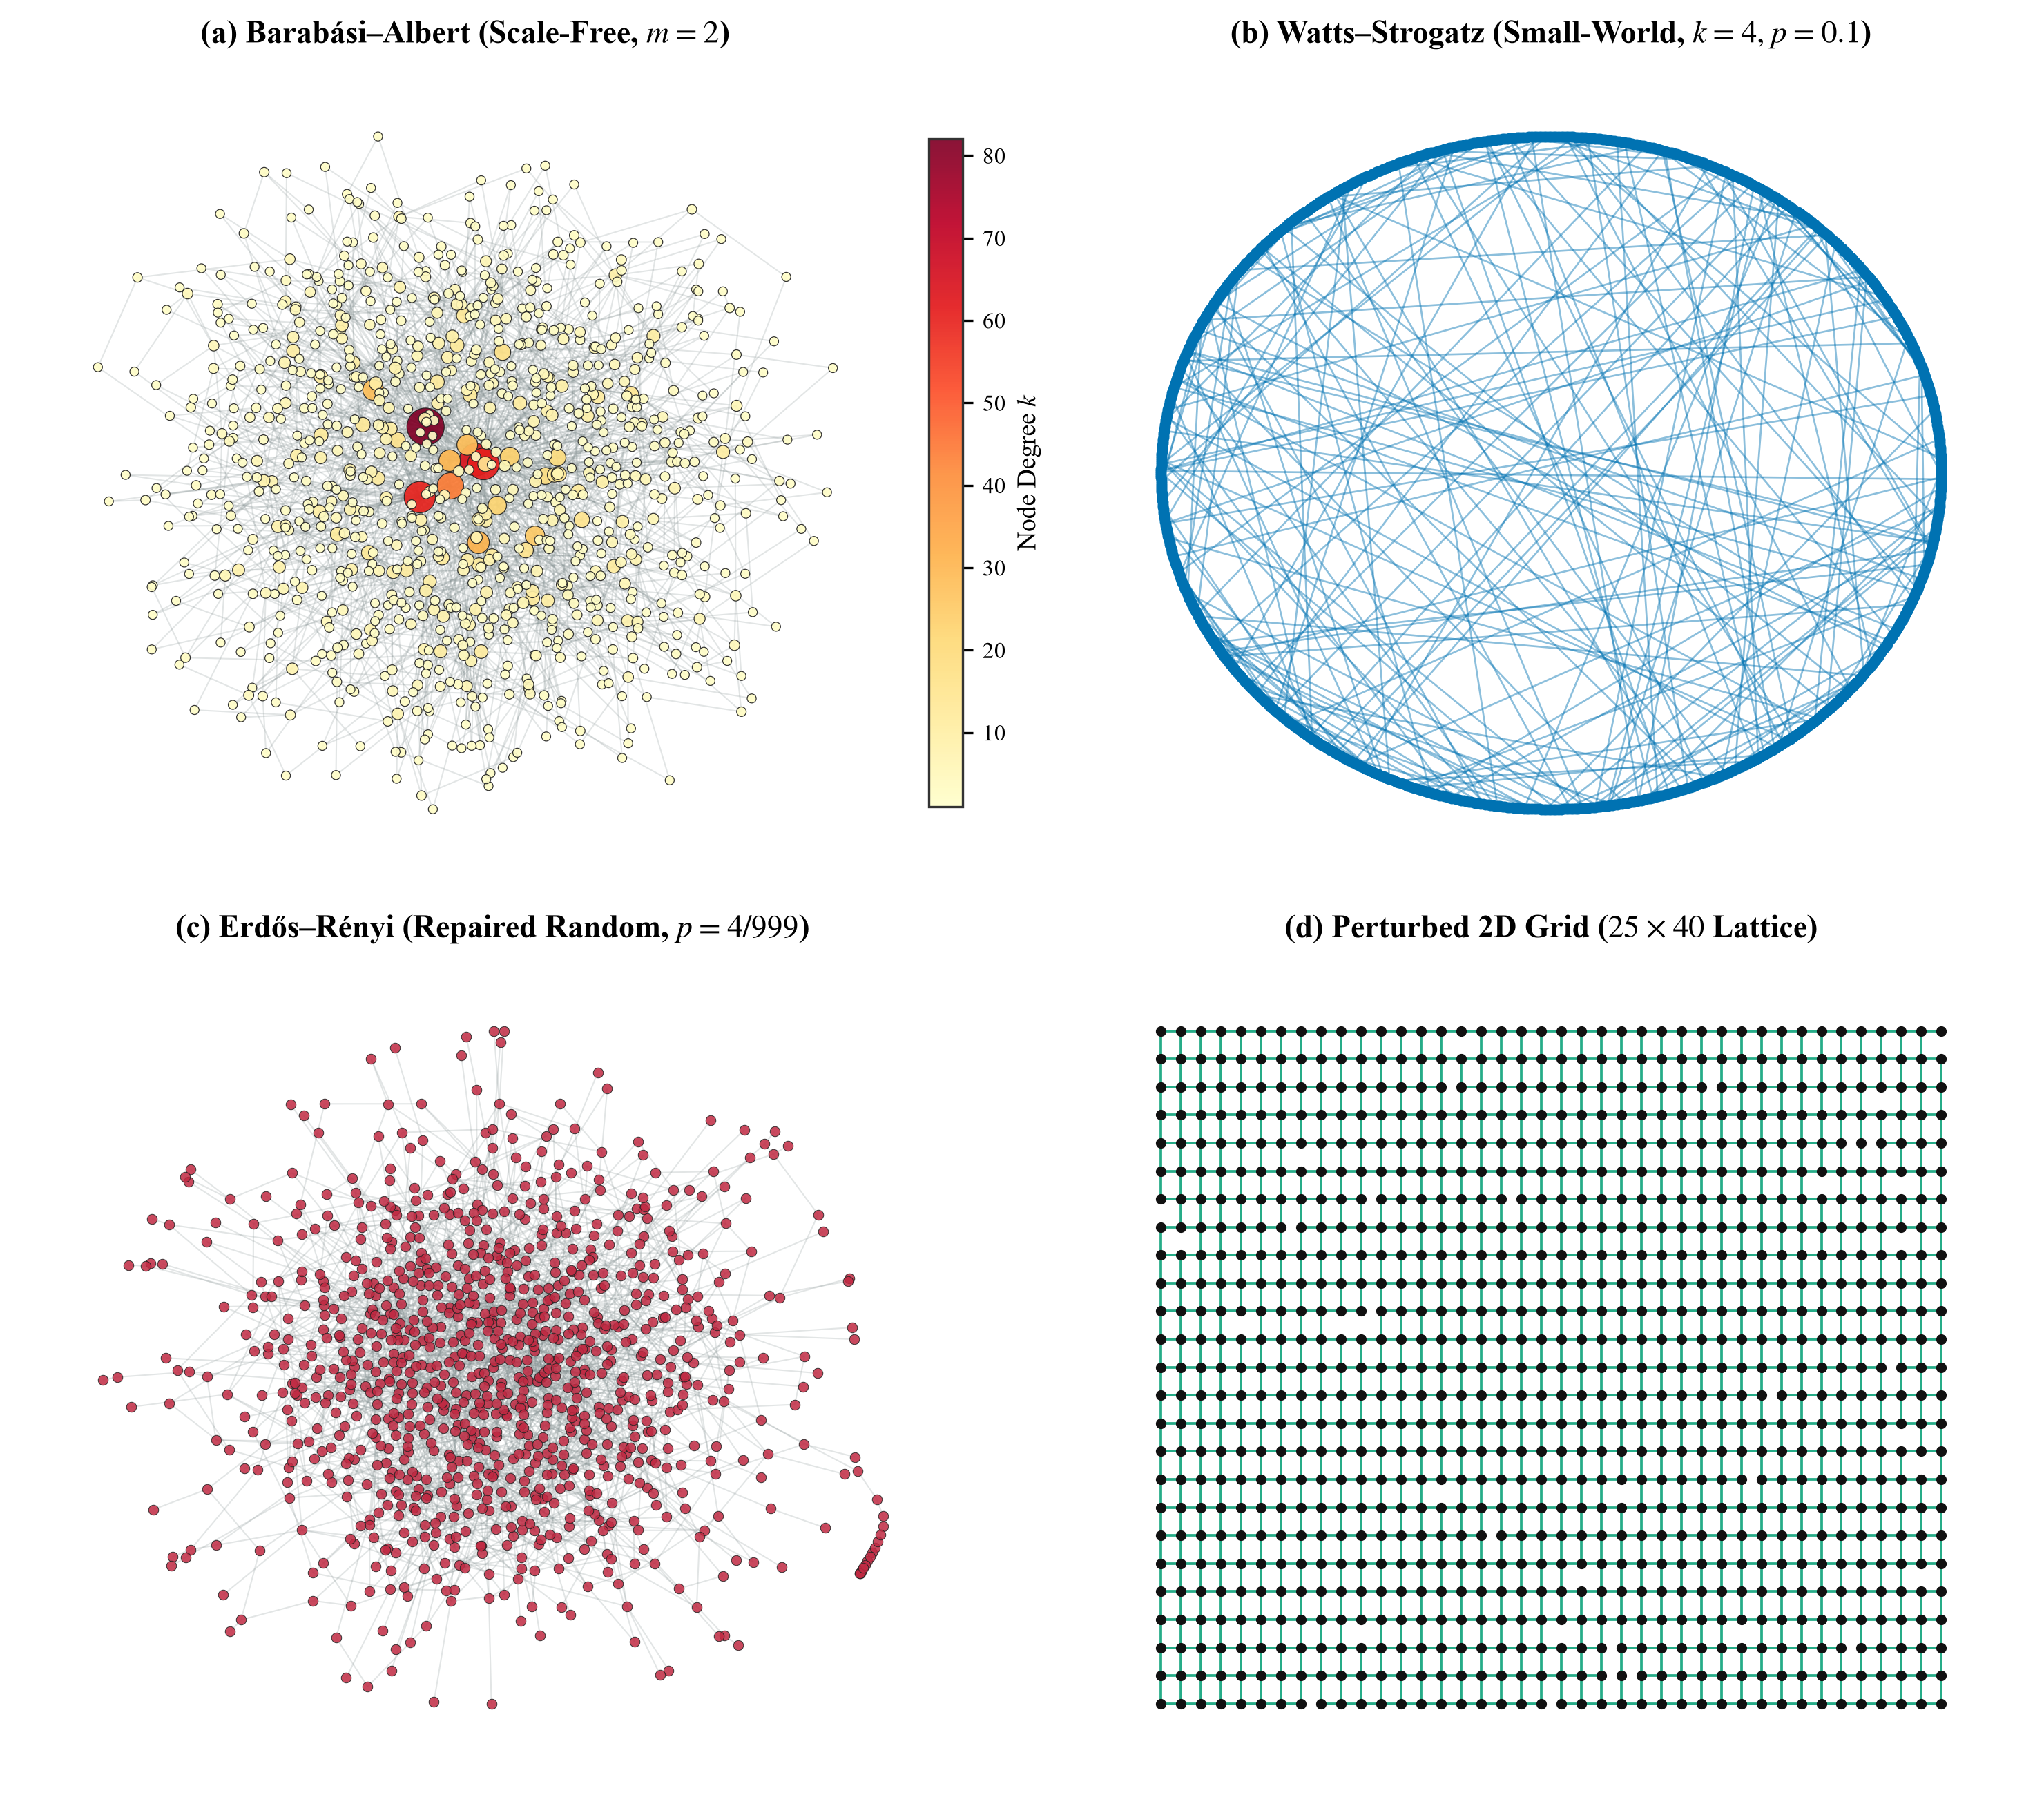
\includegraphics[width=\columnwidth]{figures/fig1_topologies.png}
    \caption{Representative instances ($N=1,000$) of the four synthetic topologies with approximately matched average degree ($\bar{d} \approx 3.8\text{--}4.0$): (a) Barab\'{a}si--Albert scale-free network, (b) Watts--Strogatz small-world network, (c) connectivity-repaired Erd\H{o}s--R\'{e}nyi random network, and (d) perturbed $25 \times 40$ planar 2D grid.}
    \label{fig:topologies}
\end{figure}

\subsection{Structural Baseline Profiling}
Before constructing spanners, each of the $120$ baseline networks is profiled to verify its structural characteristics. Five metrics are recorded for each graph:
\begin{itemize}
    \item \textit{Average Degree} ($\bar{d} = 2|E_G|/|V|$): The average number of edges connected to each vertex.
    \item \textit{Maximum Degree} ($\Delta$): The highest vertex degree, indicating the presence of highly connected hubs.
    \item \textit{Average Clustering Coefficient} ($C$): Measures the extent of local clustering through triangles ($3$-cycles).
    \item \textit{Average Shortest-Path Length} ($L$): The average shortest-path distance across all vertex pairs.
    \item \textit{Graph Diameter} ($D$): The maximum shortest-path distance between any pair of vertices.
\end{itemize}

\subsection{Greedy $t$-Spanner Construction}
For each baseline graph $G = (V, E_G)$ and target stretch factor $t \in \{3, 5, 7\}$, the standard greedy algorithm \cite{ref2} initializes an empty spanner $H = (V, \emptyset)$ containing all original vertices and inspects candidate edges $(u, v) \in E_G$ one by one. An edge is added to $H$ if and only if the current shortest-path distance between $u$ and $v$ in $H$ exceeds $t$ hops; otherwise, the edge is discarded.
Because all edges in an unweighted graph have unit weight, processing edges in a fixed generator order would introduce tie-breaking bias. To control for edge-ordering effects, the edge list $E_G$ is randomly shuffled across $10$ independent permutations per graph and stretch factor.
Across all $120$ graphs, $3$ stretch factors, and $10$ permutations ($3,600$ spanner constructions), the algorithm evaluates approximately $7.12 \times 10^6$ candidate edges. Running a full shortest-path search for each candidate edge would create a severe computational bottleneck \cite{ref23, ref22}. We therefore implement a depth-limited \textit{Bounded Breadth-First Search (Bounded BFS)} that first checks for direct adjacency or isolated endpoints in $O(1)$ time, and otherwise expands a BFS frontier from $u$ that halts strictly at depth $t$. If $v$ is reached within $t$ hops, the search terminates immediately and discards the edge; if the frontier is exhausted at depth $t$, the edge is added to $H$. Every constructed spanner undergoes an automated post-construction audit verifying that every original edge $(u, v) \in E_G$ satisfies $d_H(u, v) \le t$.

\subsection{Evaluation Metrics}
Evaluating all $\binom{1000}{2} = 499,500$ vertex pairs across $3,600$ spanners is computationally expensive. Instead, for each of the $120$ baseline graphs, we uniformly sample a fixed set of $M = 1,000$ distinct, unordered vertex pairs without replacement and cache their baseline shortest-path distances $d_G(u, v)$. Reusing the exact same $1,000$ pairs across all $t$-values and edge permutations for a given graph controls variation arising from different pair samples between experimental conditions.
For each constructed spanner $H$, shortest-path distances $d_H(u, v)$ are computed over the $1,000$ static pairs (recording any disconnected pairs as failures), and five performance metrics are evaluated:
\begin{itemize}
    \item \textit{Edge Retention Ratio:} The percentage of original edges retained in the spanner, $(|E_H| / |E_G|) \times 100\%$.
    \item \textit{Empirical Average Stretch:} The mean multiplicative stretch ratio, $\frac{1}{M} \sum (d_H(u, v) / d_G(u, v))$.
    \item \textit{Tail and Sampled Maximum Stretch:} The 95th-percentile stretch ($P_{95}$) and maximum observed stretch ($s_{\max}$) across the sampled pairs, along with the \textit{Sampled Bound Slack} ($t - s_{\max}$).
    \item \textit{Exact Maximum Stretch:} For unweighted graphs, replacing each edge along an original shortest path with its corresponding spanner detour path guarantees that the global maximum multiplicative stretch across all vertex pairs is attained on the endpoints of an original edge: $s_{\max}^{\mathrm{exact}} = \max_{(u,v)\in E_G} d_H(u,v)$. The corresponding exact bound slack is $t - s_{\max}^{\mathrm{exact}}$, establishing the true worst-case stretch independently of vertex-pair sampling.
    \item \textit{Absolute Additive Path Delay:} The mean number of extra detour hops added per path, $\frac{1}{M} \sum (d_H(u, v) - d_G(u, v))$.
    \item \textit{Construction Runtime and Order Sensitivity:} The wall-clock spanner construction time and the intra-graph standard deviation of edge retention across the $10$ edge permutations.
\end{itemize}

\subsection{Experimental Design and Statistical Analysis}
The complete experimental design comprises $4$ topologies $\times$ $30$ baseline instances $\times$ $3$ stretch limits $\times$ $10$ edge permutations, producing $3,600$ spanner runs. Treating all $300$ runs within a $(\text{topology}, t)$ condition as independent observations would commit statistical pseudoreplication by conflating within-graph permutation variance with between-graph topological variance.
To preserve the true observational unit, we apply nested aggregation: for each baseline graph and stretch factor $t$, the $10$ permutation runs are averaged into a single graph-level mean. This yields $360$ graph--stretch observations derived from the $120$ independent baseline graphs. Because each baseline graph is evaluated repeatedly across $t \in \{3, 5, 7\}$, observations across different stretch factors are dependent; however, within any fixed stretch factor $t$, the $120$ graph-level means ($n = 30$ per topology) are mutually independent.

Prior to hypothesis testing, homogeneity of variance across topologies was assessed using Levene's test. Because Levene's test demonstrated significant heteroscedasticity across topological families ($W \ge 13.60, p < 1.2 \times 10^{-7}$ for retention; $W \ge 13.11, p < 2.0 \times 10^{-7}$ for stretch), standard homoscedastic ANOVA is inappropriate. We therefore evaluate group differences using Welch’s heteroscedastic one-way ANOVA ($F_W$) \cite{ref27} alongside the non-parametric Kruskal--Wallis test ($H$, $df = 3$). Accordingly, $95\%$ confidence intervals, correlation analyses, and omnibus tests are conducted separately for each stretch factor $t$, using the graph-level means as independent observations. Pairwise comparisons between BA and GRID (RQ2) are evaluated using Welch's heteroscedastic two-sample $t$-tests (with exact Welch--Satterthwaite degrees of freedom), non-parametric Mann--Whitney $U$ tests, Cohen's $d$ effect sizes, and Student's $t$-distribution $95\%$ confidence intervals; the primary directional hypothesis ($H_{a,2}: \mu_{\mathrm{BA}} < \mu_{\mathrm{GRID}}$ on $\bar{s}$) and the directional additive-delay comparison are evaluated using one-sided tests alongside two-sided tests for magnitude quantification. Structural associations in RQ3 are assessed using Pearson correlations ($r$, with Fisher's $z$-transform $95\%$ confidence intervals) and Spearman rank correlations ($\rho$), while topological differences in sampled bound slack are tested via Welch's ANOVA ($F_W$). Multiple-testing error across hypothesis families is controlled using Holm--Bonferroni step-down and Benjamini--Hochberg False Discovery Rate (FDR) adjustments.

% ============================================================================
% SECTION VI: RESULTS AND DISCUSSION
% ============================================================================
\section{Results and Discussion}

\subsection{Baseline Structural Profiling and Validation}

Table~\ref{tab:baseline_profiles} summarizes the baseline structural profiles across all $120$ generated networks ($n = 30$ independent instances per topology at $N = 1,000$ vertices). The profiling results confirm that baseline edge density is closely matched across the four generators ($\bar{d} \approx 3.79\text{--}4.04$), while the remaining structural metrics separate the networks into four distinct topological regimes:

\begin{itemize}
    \item \textit{Barab\'{a}si--Albert (BA):} Exhibits a heavy-tailed, right-skewed degree distribution consistent with preferential attachment, producing prominent central hubs (average $\Delta = 84.1$, reaching up to $116$) that compress the baseline network to the shortest average path length ($L = 4.06$) and smallest diameter ($D = 7.2$).
    \item \textit{Watts--Strogatz (WS):} Maintains tightly bounded vertex degrees ($\Delta \le 8$) while achieving a clustering coefficient ($C = 0.3735$) more than two orders of magnitude higher than ER and over $14\times$ higher than BA, confirming dense local triangle closure alongside moderate path lengths ($L = 8.80$).
    \item \textit{Erd\H{o}s--R\'{e}nyi (ER):} Exhibits a narrow degree range ($\Delta = 12.1 \pm 1.4$), short path lengths ($L = 5.37$), and near-zero clustering ($C = 0.0036 \approx p$), reflecting a locally tree-like structure with very few triangles (with mandatory bridge edges accounting for $< 5\%$ of $|E_G|$, as established in Section~V-A).
    \item \textit{Perturbed 2D Grid (GRID):} Represents a strictly bipartite planar lattice ($C = 0$, minimum cycle length of $4$) with uniform maximum degree ($\Delta = 4.0$) and an average path length ($L = 21.70$) more than five times longer than BA.
\end{itemize}

Furthermore, across all $3,600$ constructed spanners, the automated post-construction audit confirmed $100\%$ compliance with the spanner invariant ($d_H(u, v) \le t$ for every $(u, v) \in E_G$) and recorded zero disconnected vertex pairs across all $3.6 \times 10^6$ evaluated pair queries, verifying that the greedy algorithm strictly preserves global connectivity \cite{ref1, ref2}.

\begin{table*}[t]
\centering
\caption{Baseline Structural Profiles Across Topological Families ($n = 30$ Independent Instances Per Topology, $N = 1,000$ Vertices)}
\label{tab:baseline_profiles}
\footnotesize
\setlength{\tabcolsep}{4pt}
\renewcommand{\arraystretch}{1.15}

\resizebox{\textwidth}{!}{%
\begin{tabular}{@{}lcccccc@{}}
\toprule
\textbf{Topology Family} & \textbf{Edges ($|E_G|$)} & \textbf{Avg.\ Degree ($\bar{d}$)} & \textbf{Max Degree ($\Delta$)} & \textbf{Clustering Coeff.\ ($C$)} & \textbf{Avg.\ Path Length ($L$)} & \textbf{Diameter ($D$)} \\
\midrule
Barab\'{a}si--Albert (BA) & $1996.0 \pm 0.0$ & $3.99 \pm 0.00$ & $84.1 \pm 13.8$ & $0.0261 \pm 0.0070$ & $4.06 \pm 0.06$ & $7.2 \pm 0.4$ \\
Watts--Strogatz (WS) & $2000.0 \pm 0.0$ & $4.00 \pm 0.00$ & $6.7 \pm 0.6$ & $0.3735 \pm 0.0085$ & $8.80 \pm 0.24$ & $17.7 \pm 1.4$ \\
Erd\H{o}s--R\'{e}nyi (ER) & $2018.8 \pm 37.4$ & $4.04 \pm 0.07$ & $12.1 \pm 1.4$ & $0.0036 \pm 0.0013$ & $5.37 \pm 0.17$ & $25.0 \pm 4.5$ \\
Perturbed 2D Grid (GRID) & $1896.0 \pm 0.0$ & $3.79 \pm 0.00$ & $4.0 \pm 0.0$ & $0.0000 \pm 0.0000$ & $21.70 \pm 0.01$ & $63.0 \pm 0.0$ \\
\bottomrule
\end{tabular}%
}
\end{table*}

\subsection{Topological Effect on Edge Sparsity and Path Stretch (RQ1)}

Table~\ref{tab:main_results} reports the nested graph-level performance metrics across all four topologies and stretch factors $t \in \{3, 5, 7\}$.

\begin{table*}[t]
\centering
\caption{Empirical Greedy $t$-Spanner Performance Across Topologies and Stretch Factors ($n = 30$ Nested Graph-Level Means $\pm$ SD). Sampled Max Stretch and Bound Slack are evaluated over $M = 1,000$ uniformly sampled vertex pairs; across all $3,600$ constructed spanners, exact edge-level maximum stretch strictly attains $t$ ($s_{\max}^{\text{exact}} = t$, exact edge bound slack $= 0.00$). Additive path delay reports true pairwise extra hops $\mathbb{E}[d_H(u,v) - d_G(u,v)]$.}
\label{tab:main_results}
\footnotesize
\setlength{\tabcolsep}{3pt}
\renewcommand{\arraystretch}{1.15}

\resizebox{\textwidth}{!}{%
\begin{tabular}{@{}lcrrrrrrr@{}}
\toprule
\textbf{Topology} & \textbf{$t$} & \textbf{Retained (\%)} & \textbf{Avg.\ Stretch ($\bar{s}$)} & \textbf{$P_{95}$ Stretch} & \textbf{Mean Sampled Max.\ ($s_{\max}$)} & \textbf{Mean Sampled Slack ($t - s_{\max}$)} & \textbf{Add.\ Delay (Hops)} & \textbf{Runtime (ms)} \\
\midrule
(BA) & $3$ & $91.7 \pm 0.7$ & $1.097 \pm 0.010$ & $1.453 \pm 0.045$ & $2.41 \pm 0.24$ & $0.59 \pm 0.24$ & $+0.34 \pm 0.03$ & $20.3 \pm 2.7$ \\
 & $5$ & $75.9 \pm 0.8$ & $1.329 \pm 0.017$ & $1.998 \pm 0.008$ & $4.01 \pm 0.29$ & $0.99 \pm 0.29$ & $+1.19 \pm 0.04$ & $59.8 \pm 5.9$ \\
 & $7$ & $64.6 \pm 0.6$ & $1.602 \pm 0.020$ & $2.423 \pm 0.074$ & $5.46 \pm 0.56$ & $1.54 \pm 0.56$ & $+2.22 \pm 0.04$ & $86.4 \pm 7.4$ \\
\midrule
(WS) & $3$ & $65.9 \pm 0.5$ & $1.168 \pm 0.006$ & $1.429 \pm 0.013$ & $2.39 \pm 0.25$ & $0.61 \pm 0.25$ & $+1.42 \pm 0.08$ & $4.6 \pm 1.1$ \\
 & $5$ & $60.8 \pm 0.6$ & $1.247 \pm 0.009$ & $1.590 \pm 0.015$ & $3.14 \pm 0.39$ & $1.86 \pm 0.39$ & $+2.07 \pm 0.13$ & $5.5 \pm 1.2$ \\
 & $7$ & $59.6 \pm 0.6$ & $1.281 \pm 0.010$ & $1.661 \pm 0.019$ & $3.41 \pm 0.48$ & $3.59 \pm 0.48$ & $+2.35 \pm 0.13$ & $6.9 \pm 1.4$ \\
\midrule
(ER) & $3$ & $98.0 \pm 0.3$ & $1.012 \pm 0.003$ & $1.043 \pm 0.051$ & $1.79 \pm 0.17$ & $1.21 \pm 0.17$ & $+0.05 \pm 0.01$ & $8.9 \pm 2.0$ \\
 & $5$ & $88.5 \pm 0.7$ & $1.105 \pm 0.006$ & $1.494 \pm 0.010$ & $3.45 \pm 0.53$ & $1.55 \pm 0.53$ & $+0.47 \pm 0.02$ & $35.1 \pm 4.4$ \\
 & $7$ & $75.4 \pm 1.1$ & $1.309 \pm 0.015$ & $1.969 \pm 0.042$ & $5.34 \pm 0.64$ & $1.66 \pm 0.64$ & $+1.41 \pm 0.05$ & $69.2 \pm 7.7$ \\
\midrule
(GRID) & $3$ & $72.7 \pm 0.1$ & $1.071 \pm 0.003$ & $1.289 \pm 0.008$ & $2.63 \pm 0.26$ & $0.37 \pm 0.26$ & $+1.17 \pm 0.06$ & $7.2 \pm 1.4$ \\
 & $5$ & $64.7 \pm 0.1$ & $1.141 \pm 0.004$ & $1.434 \pm 0.014$ & $3.47 \pm 0.38$ & $1.53 \pm 0.38$ & $+2.38 \pm 0.09$ & $9.0 \pm 1.6$ \\
 & $7$ & $60.8 \pm 0.1$ & $1.210 \pm 0.006$ & $1.565 \pm 0.015$ & $4.42 \pm 0.54$ & $2.58 \pm 0.54$ & $+3.64 \pm 0.11$ & $10.1 \pm 2.0$ \\
\bottomrule
\end{tabular}%
}
\end{table*}

Fig.~\ref{fig:avg_stretch} and Fig.~\ref{fig:tail_stretch} illustrate how path distortion evolves across the $30$ instances per family as $t$ increases. At $t = 3$, ER exhibits almost no distortion (Fig.~\ref{fig:avg_stretch}) because nearly all of its original edges are retained, whereas WS shows the highest initial average stretch ($1.168$) due to aggressive early pruning. As the stretch budget relaxes to $t = 5$ and $t = 7$, however, BA experiences the steepest growth in both average stretch (Fig.~\ref{fig:avg_stretch}) and 95th-percentile tail stretch (Fig.~\ref{fig:tail_stretch}), reaching $\bar{s} = 1.602$ and $P_{95} = 2.423$ at $t=7$. In contrast, GRID exhibits modest distortion growth across $t$, achieving the lowest tail stretch at $t=5$ ($1.434$) and $t=7$ ($1.565$), as well as the lowest average stretch at $t=7$ ($1.210$, whereas ER achieves the lowest average stretch at $t=5$ with $1.105$), with minimal variance across instances.

\begin{figure}[!t]
    \centering
    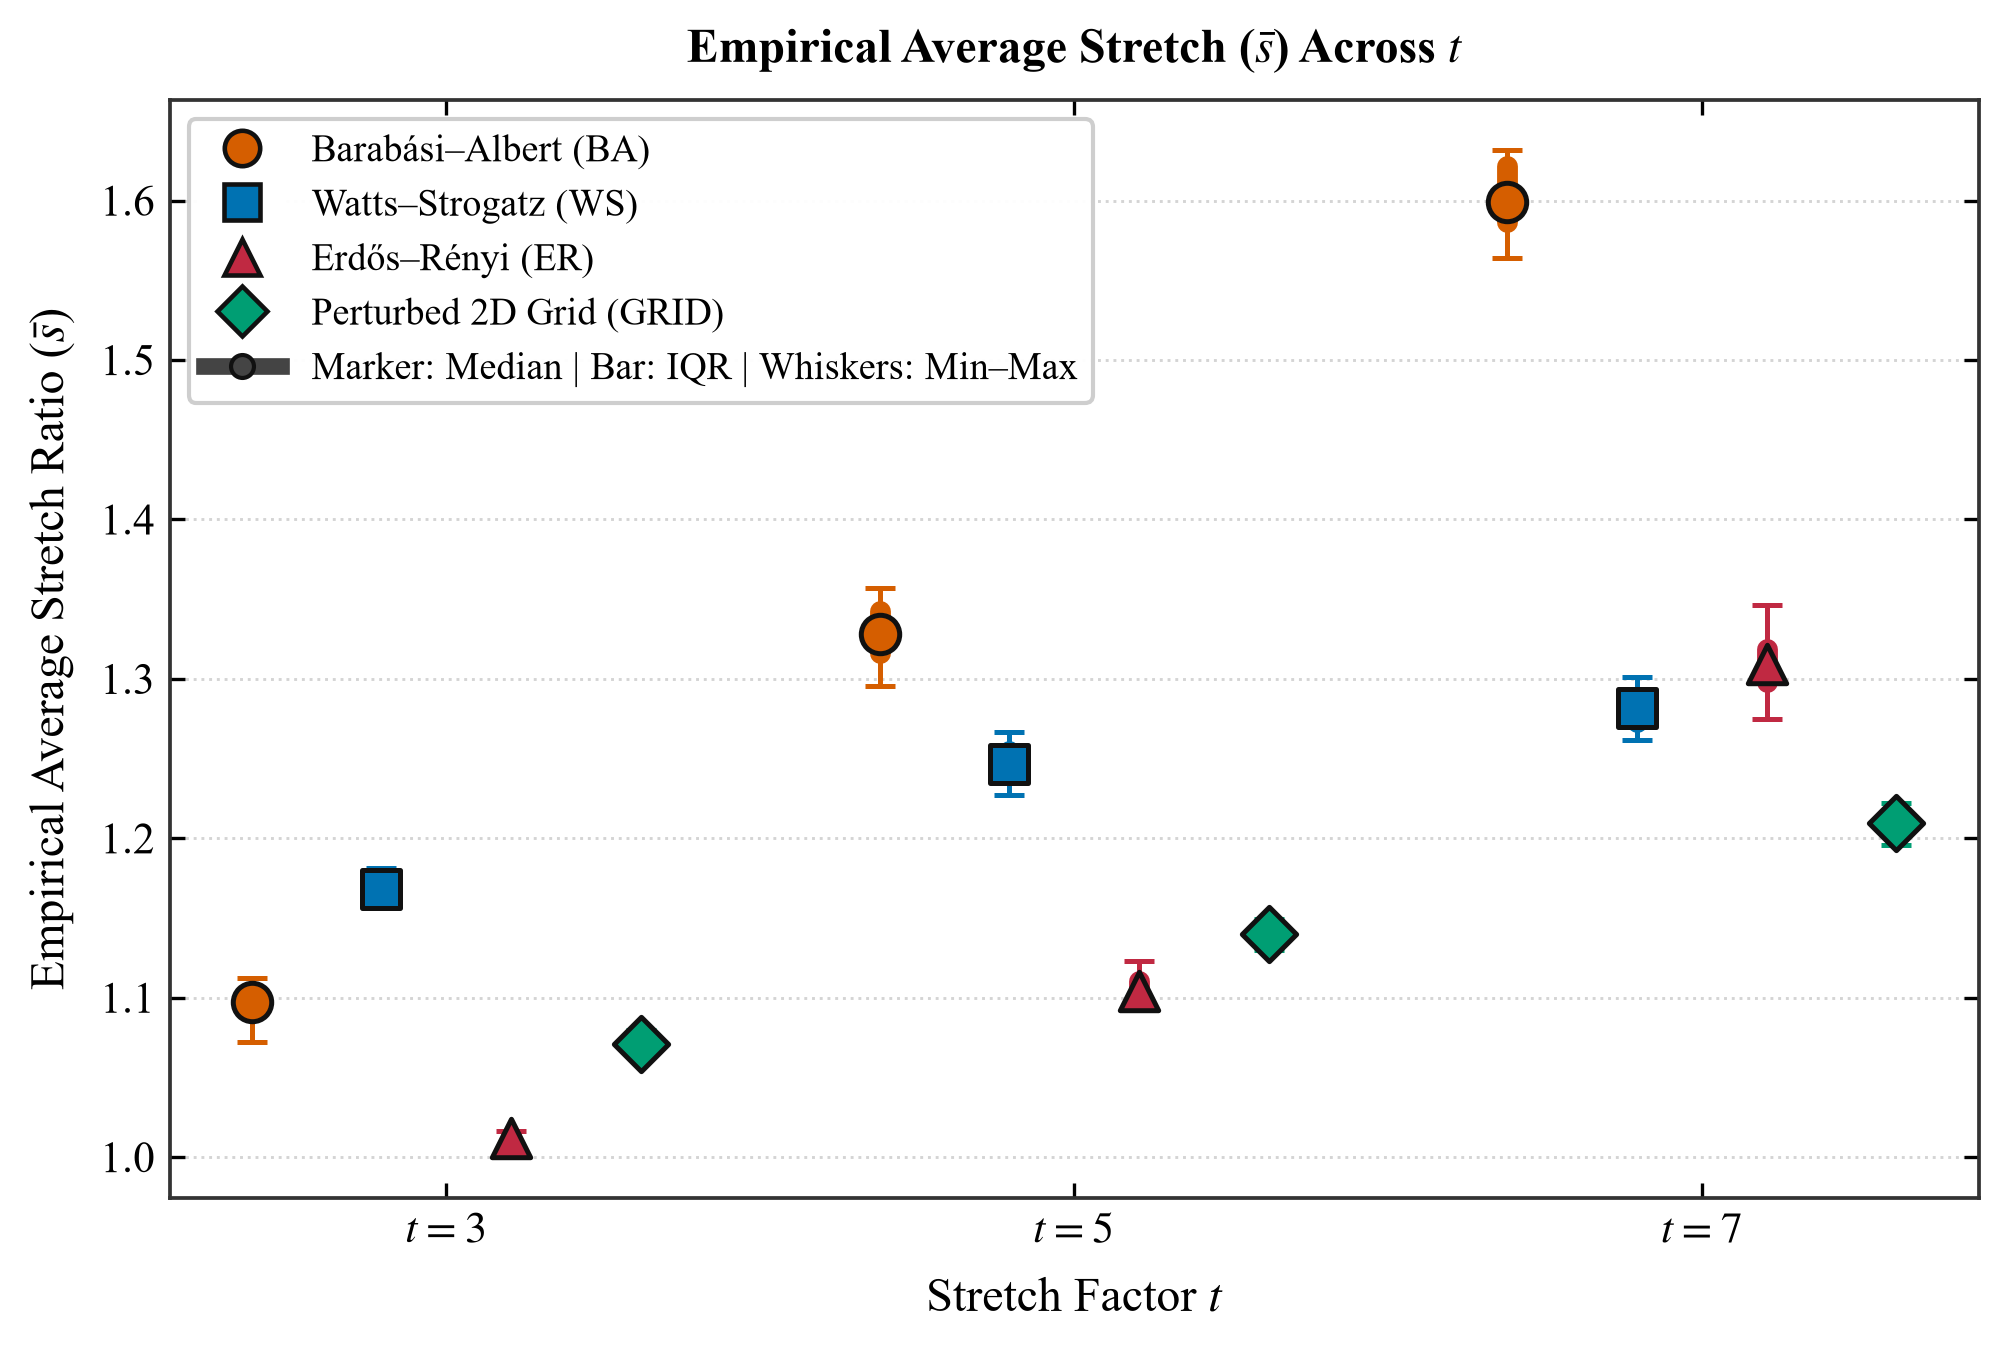
\includegraphics[width=\columnwidth]{figures/fig3_stretch_distributions.png}
    \caption{Empirical average stretch ratio ($\bar{s}$) across stretch factors $t \in \{3, 5, 7\}$ ($n = 30$ independent graph instances per topology). Marker: Median; thick bar: IQR; whiskers: Min--Max range.}
    \label{fig:avg_stretch}
\end{figure}

\begin{figure}[!t]
    \centering
    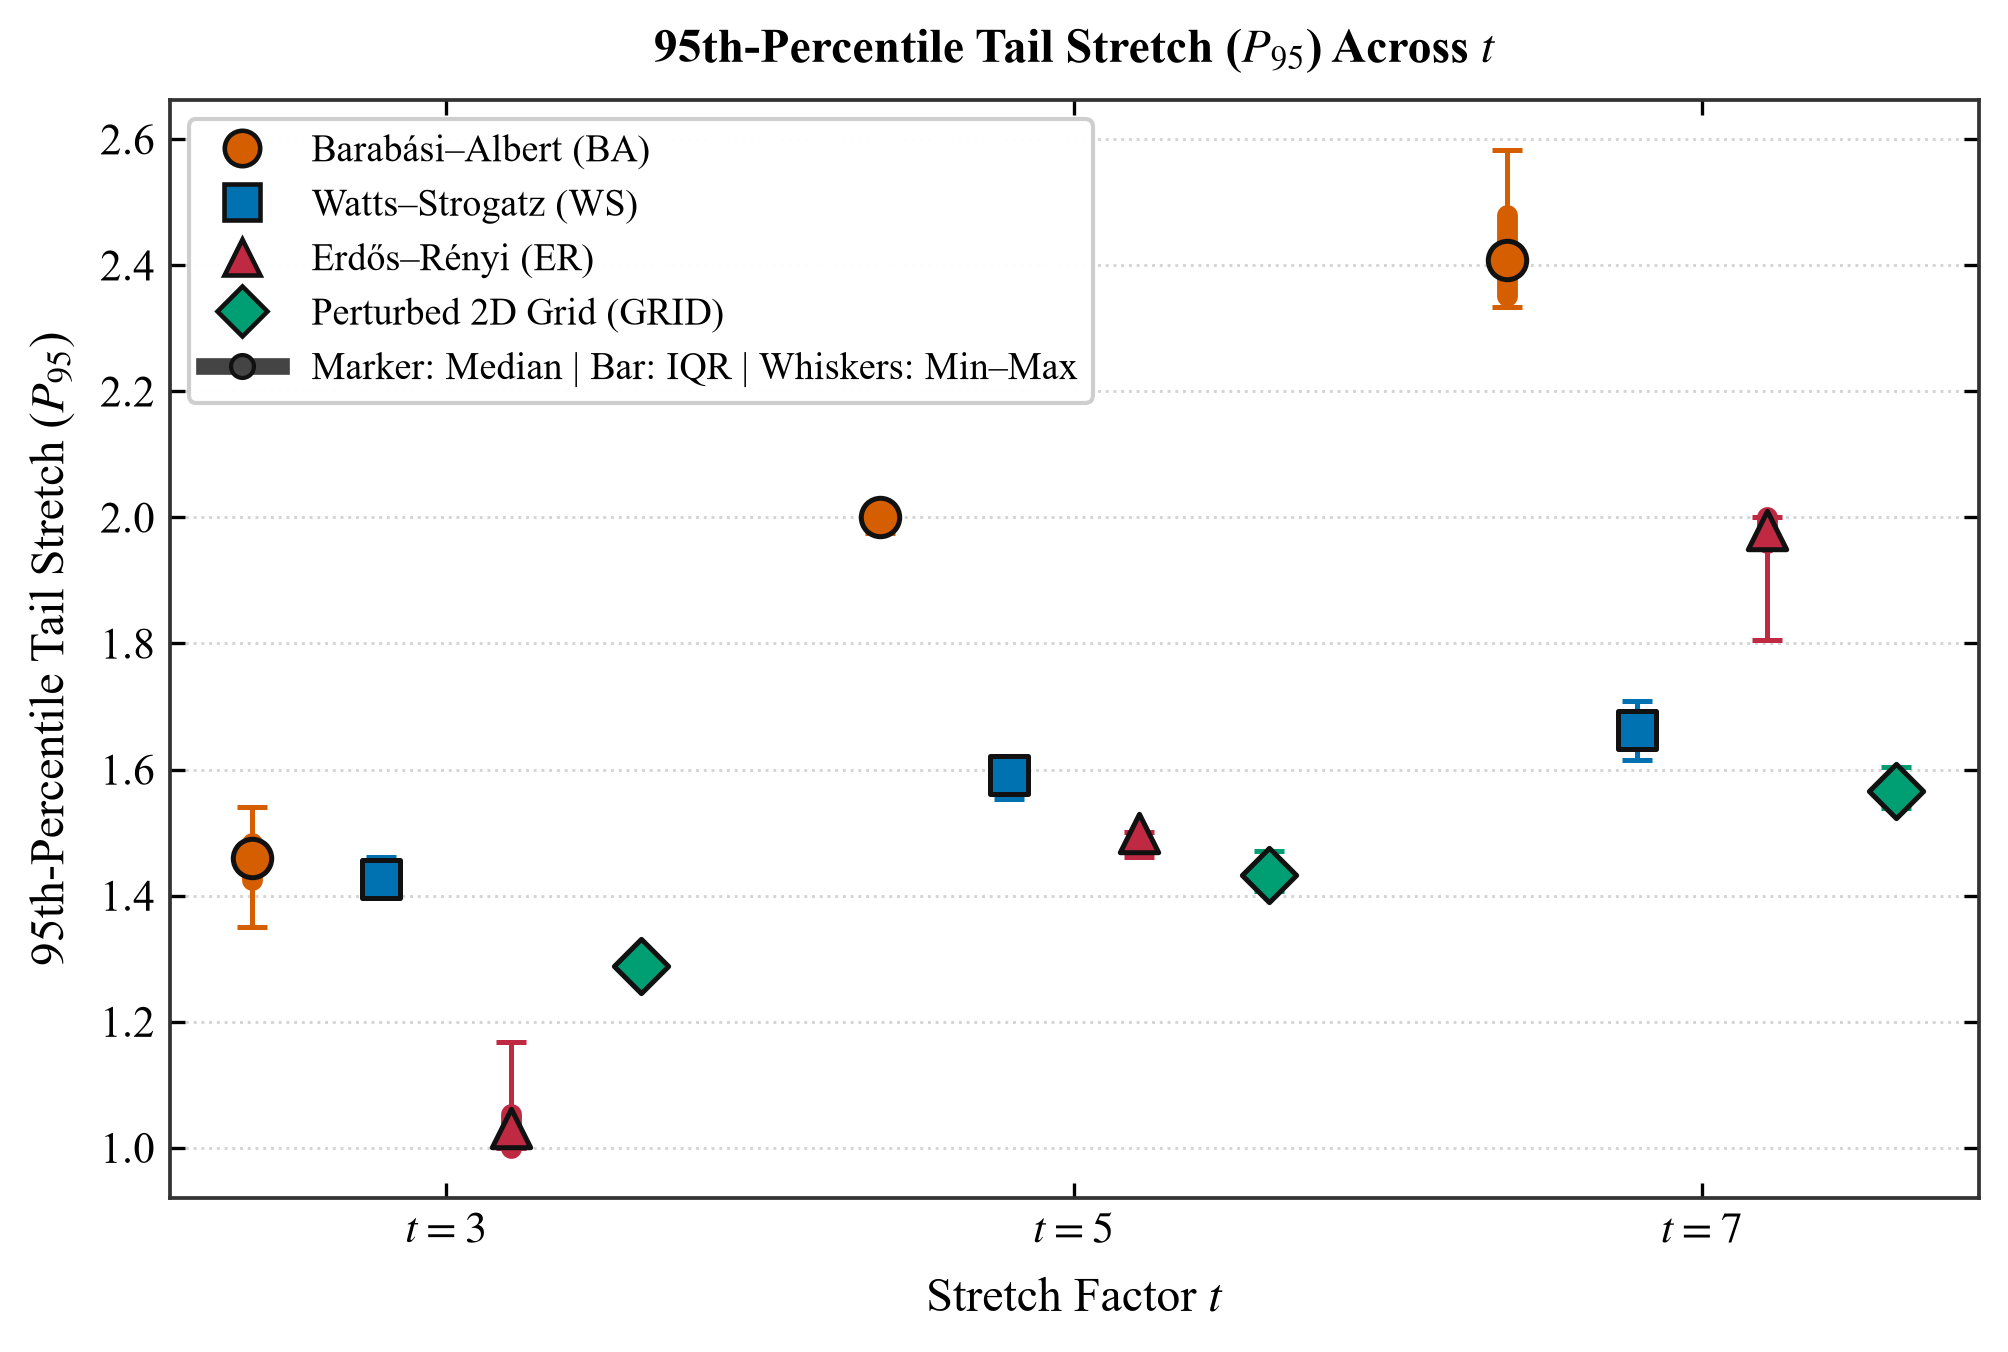
\includegraphics[width=\columnwidth]{figures/fig3_stretch_distributions_95th.png}
    \caption{95th-percentile tail stretch ($P_{95}$) across stretch factors $t \in \{3, 5, 7\}$ ($n = 30$ independent graph instances per topology). Marker: Median; thick bar: IQR; whiskers: Min--Max range.}
    \label{fig:tail_stretch}
\end{figure}

Fig.~\ref{fig:edge_retention} reveals three distinct sparsification patterns across $t$. First, WS (blue dashed curve) prunes over a third of its edges immediately at $t=3$ ($65.9\%$ retained), but shows strong diminishing returns beyond $t=3$, losing only $6.3$ additional percentage points up to $t=7$ ($59.6\%$) as it approaches the spanning-tree connectivity lower bound ($(N-1)/|E_G| \approx 50\%$ for $\bar{d} \approx 4.0$). Second, GRID (green dotted curve) thins steadily from $72.7\%$ to $60.8\%$, achieving lower retention than both BA and ER across all $t$ despite starting with a slightly lower baseline degree ($\bar{d} = 3.79$). Third, ER and BA resist pruning at $t=3$ ($98.0\%$ and $91.7\%$ retained, with over $97.9\%$ of ER's non-bridge cyclic edges remaining unpruned even after accounting for its $4.97\%$ mandatory bridge edges), but drop steeply once $t \ge 5$ allows longer cycles to be broken.

\begin{figure}[!t]
    \centering
    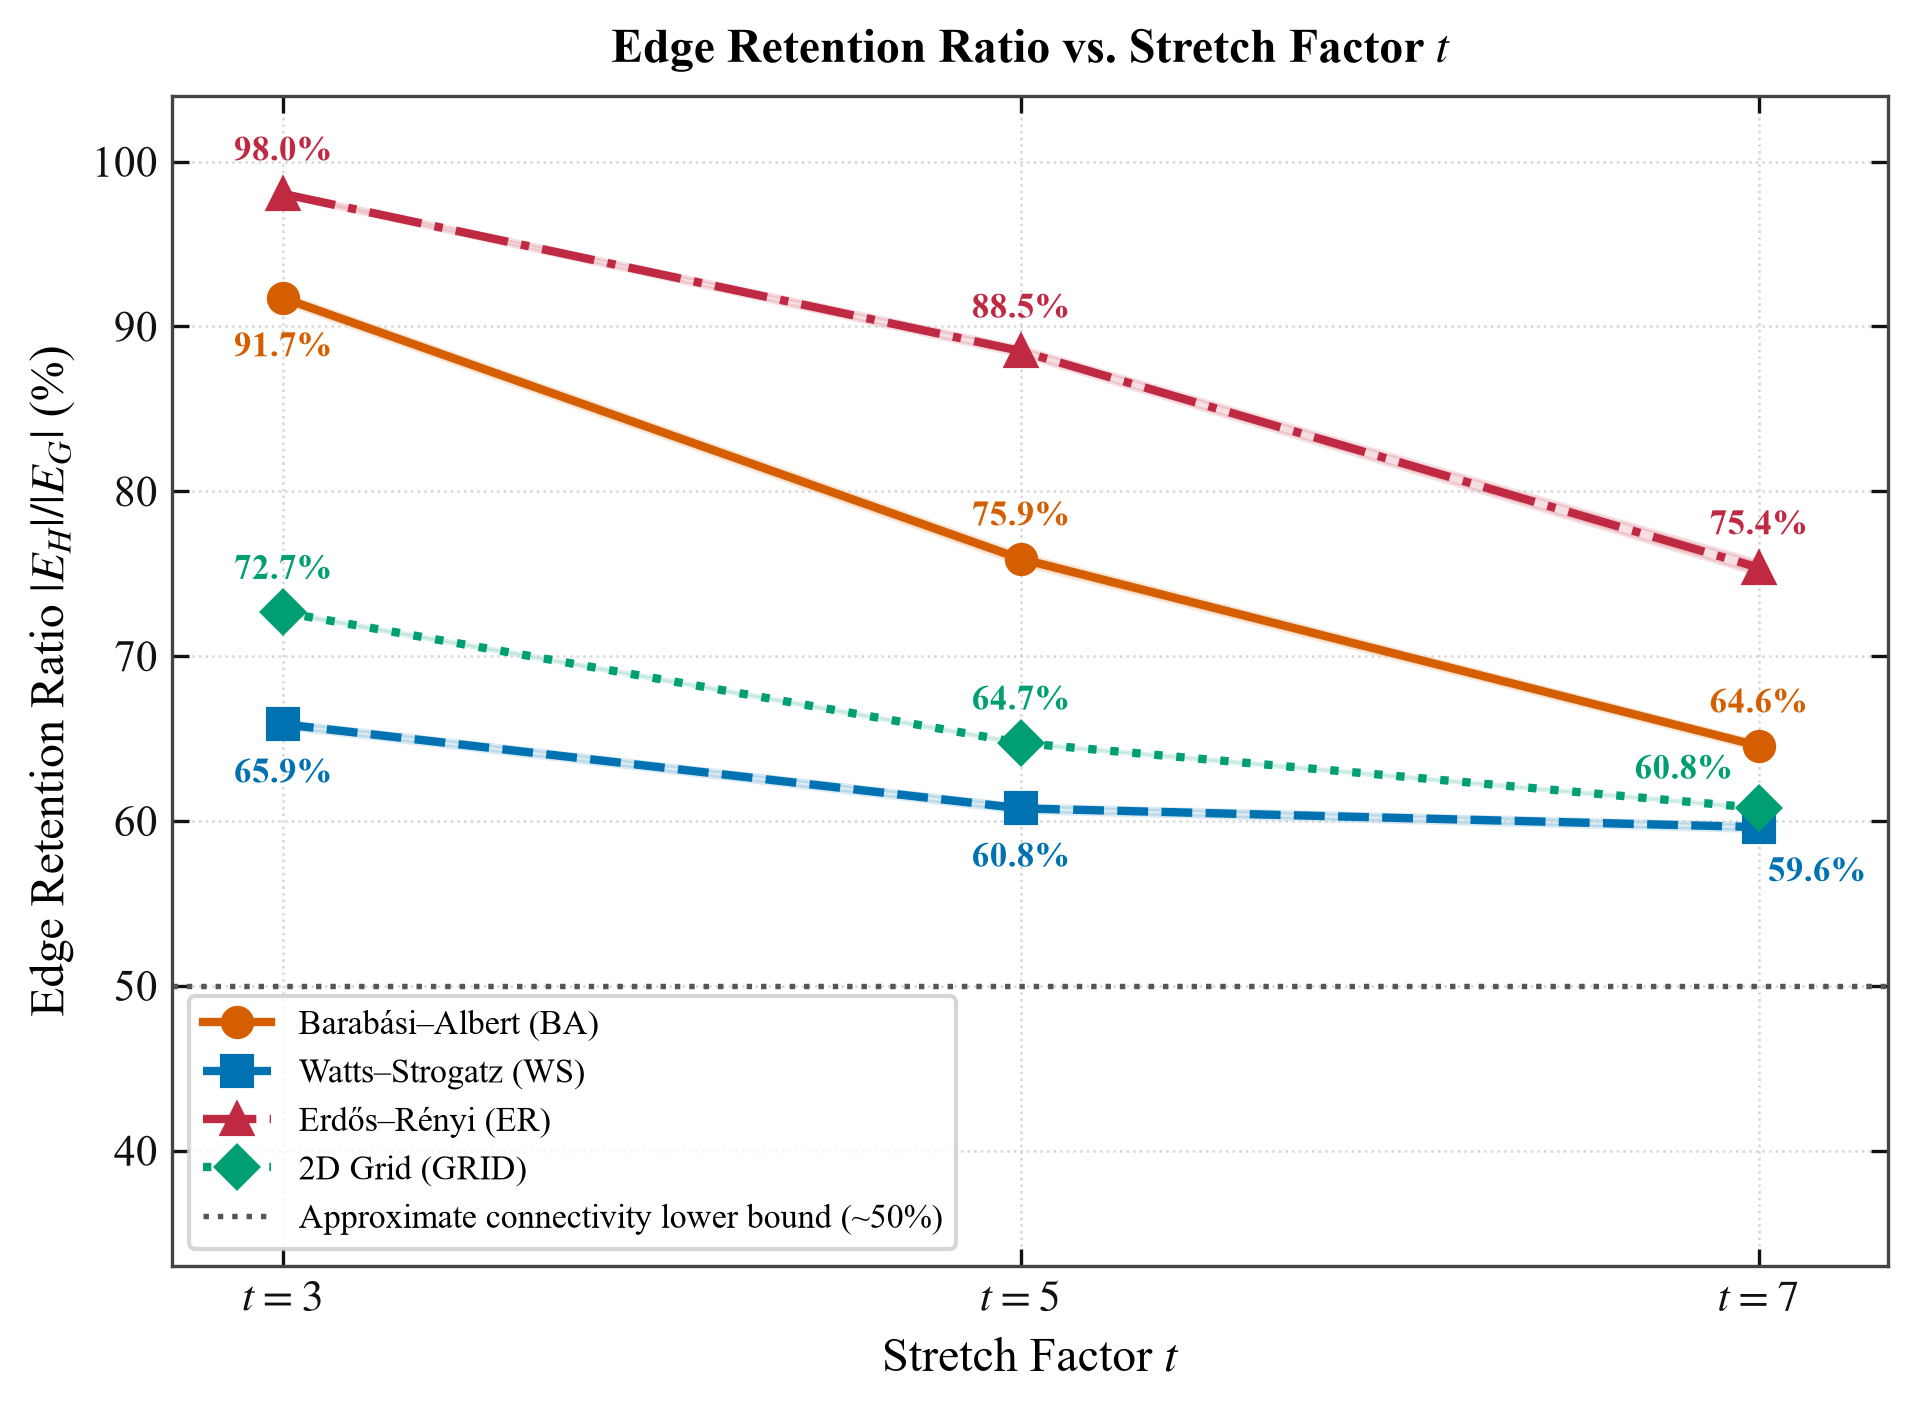
\includegraphics[width=\columnwidth]{figures/fig4_sparsity.png}
    \caption{Mean edge retention ratio $|E_H|/|E_G|$ (\%) with $95\%$ confidence intervals versus stretch factor $t$, relative to the approximate connectivity lower bound ($\approx 50\%$).}
    \label{fig:edge_retention}
\end{figure}

Plotting both objectives together on the multi-objective stretch--sparsity trade-off landscape (Fig.~\ref{fig:pareto_frontier}) demonstrates that GRID strictly dominates BA across every stretch factor $t \in \{3, 5, 7\}$ by achieving both lower edge retention and lower average stretch. Across the entire experimental design space, the non-dominated Pareto frontier is formed by the outer envelope spanning ER at $t=3$ (lowest overall stretch, $\bar{s} = 1.012$), GRID across all $t$, and WS at $t=7$ (highest overall sparsity, $59.6\%$ retention). Furthermore, while WS trades slightly higher average stretch ($1.168$ vs.\ $1.097$) for much greater sparsity ($65.9\%$ vs.\ $91.7\%$) relative to BA at $t=3$, WS dominates BA at both $t=5$ and $t=7$.

\begin{figure}[!t]
    \centering
    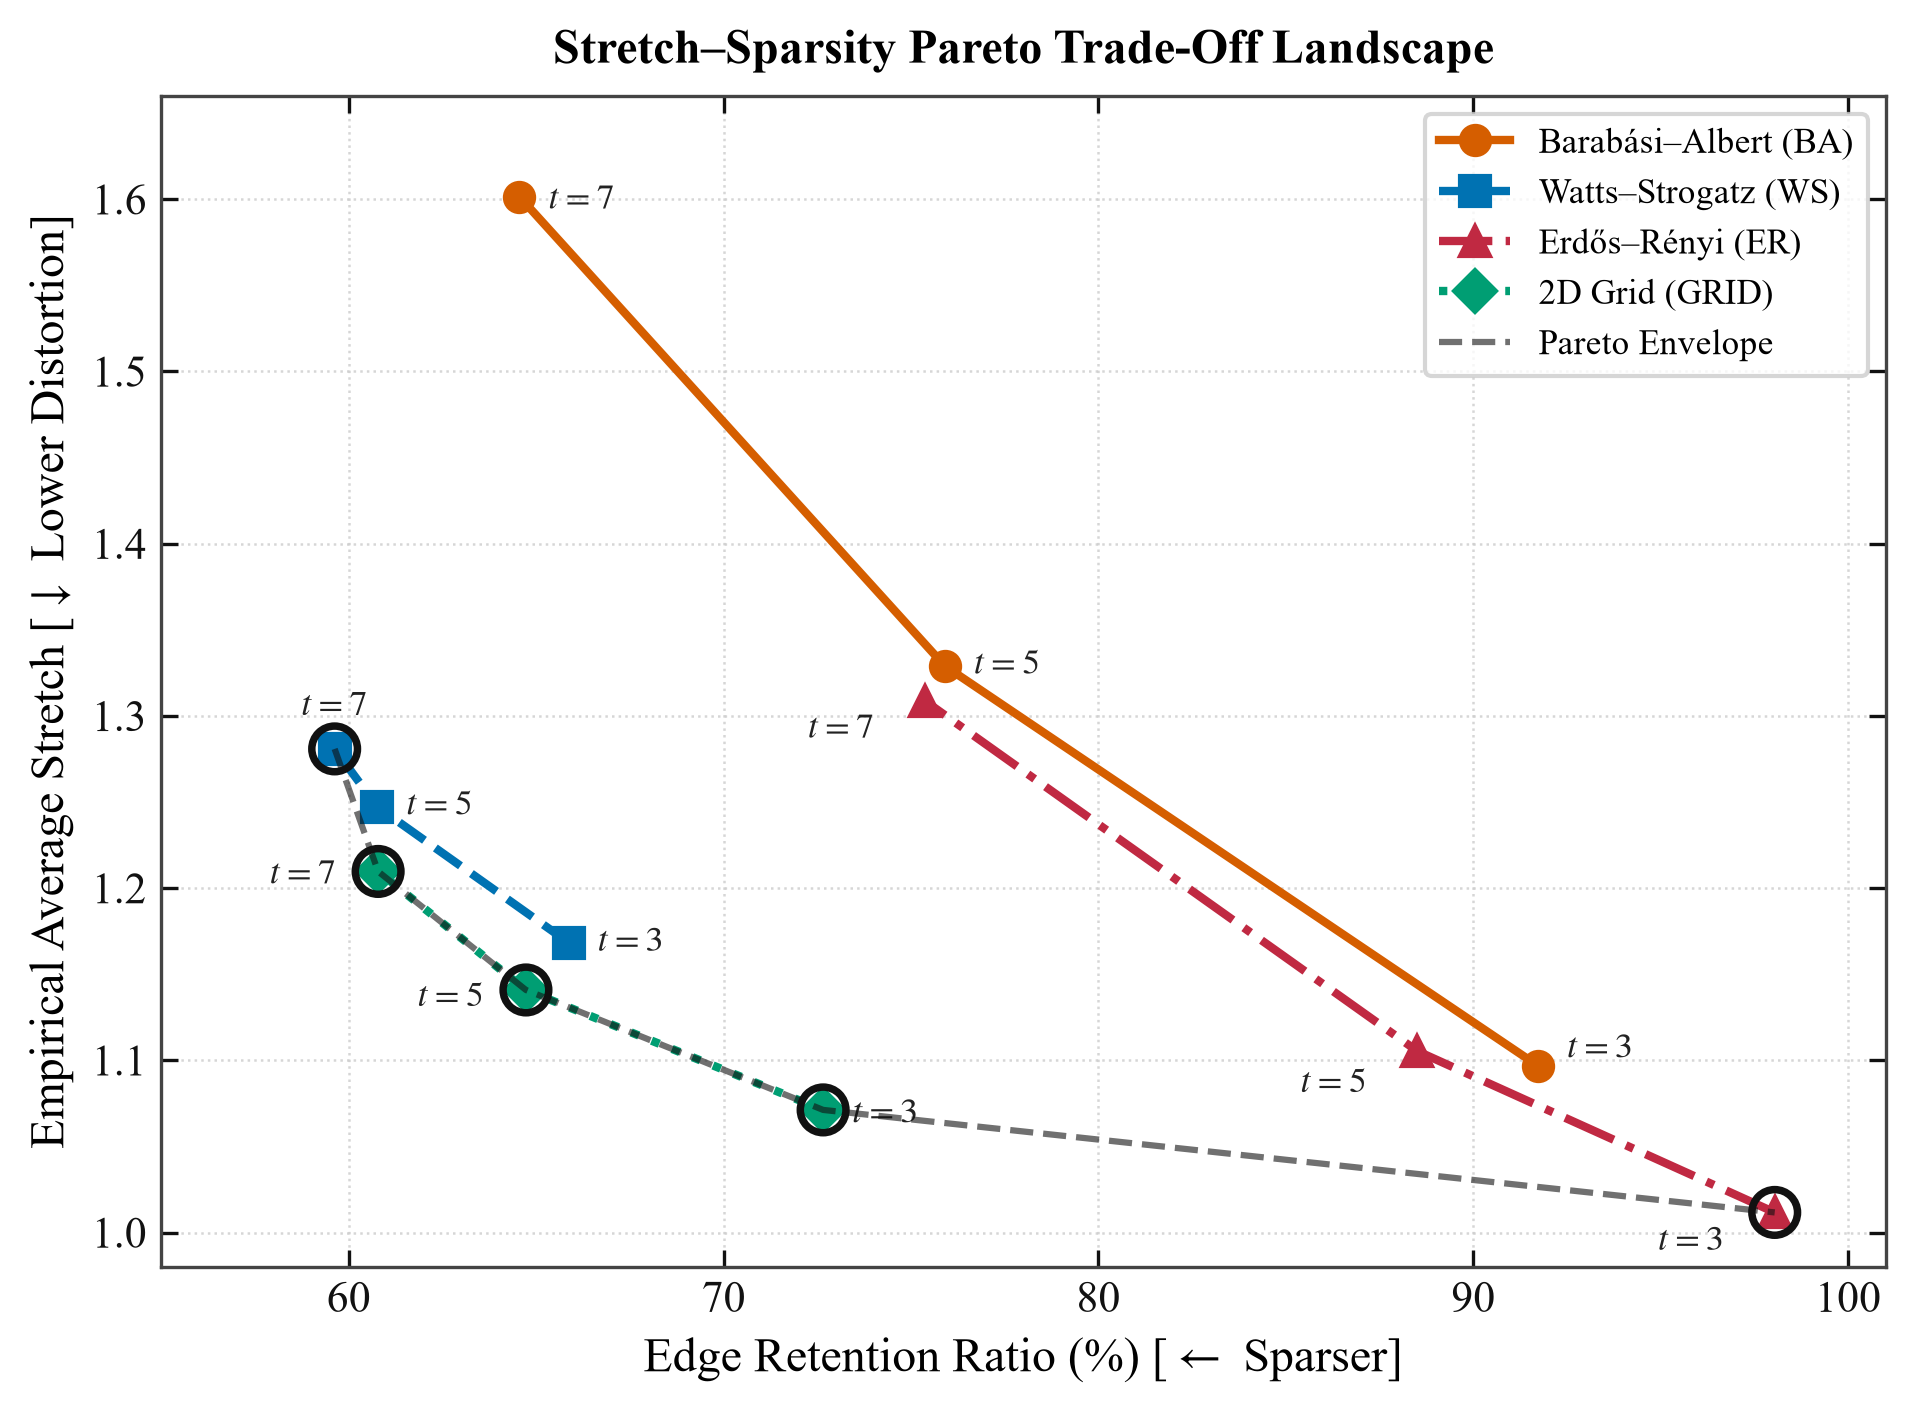
\includegraphics[width=\columnwidth]{figures/fig4_pareto.png}
    \caption{Empirical stretch--sparsity Pareto trade-off frontier across stretch factors $t \in \{3, 5, 7\}$ (lower edge retention and lower stretch represent superior performance). Circled points indicate non-dominated configurations along the Pareto envelope; connecting lines are visual guides across $t$.}
    \label{fig:pareto_frontier}
\end{figure}

Reflecting these systematic behavioral divergences, Welch's heteroscedastic one-way ANOVA on the $n = 30$ independent graph-level means (confirmed non-parametrically via Kruskal--Wallis, $p < 10^{-22}$) confirms that topological differences are highly statistically significant across all stretch factors for both edge retention ($F_W \ge 2,216.4, p < 10^{-51}$) and empirical average stretch ($F_W \ge 2,752.4, p < 10^{-63}$). We therefore reject $H_{0,1}$ in favor of $H_{a,1}$: underlying network topology strongly governs both spanner sparsity and path distortion.

\subsection{Scale-Free Hubs vs.\ Planar Grids: Multiplicative Stretch vs.\ Additive Delay (RQ2)}

To address RQ2 and test $H_{0,2}$, whether scale-free hubs (BA) protect path lengths from severe stretching compared to rigid planar grids (GRID), we compare the same spanner runs using two complementary distance metrics: multiplicative relative stretch ($d_H / d_G$, Fig.~\ref{fig:multiplicative_stretch}) and absolute additive path delay ($d_H - d_G$ in hops, Fig.~\ref{fig:additive_delay}).

\begin{figure}[!t]
    \centering
    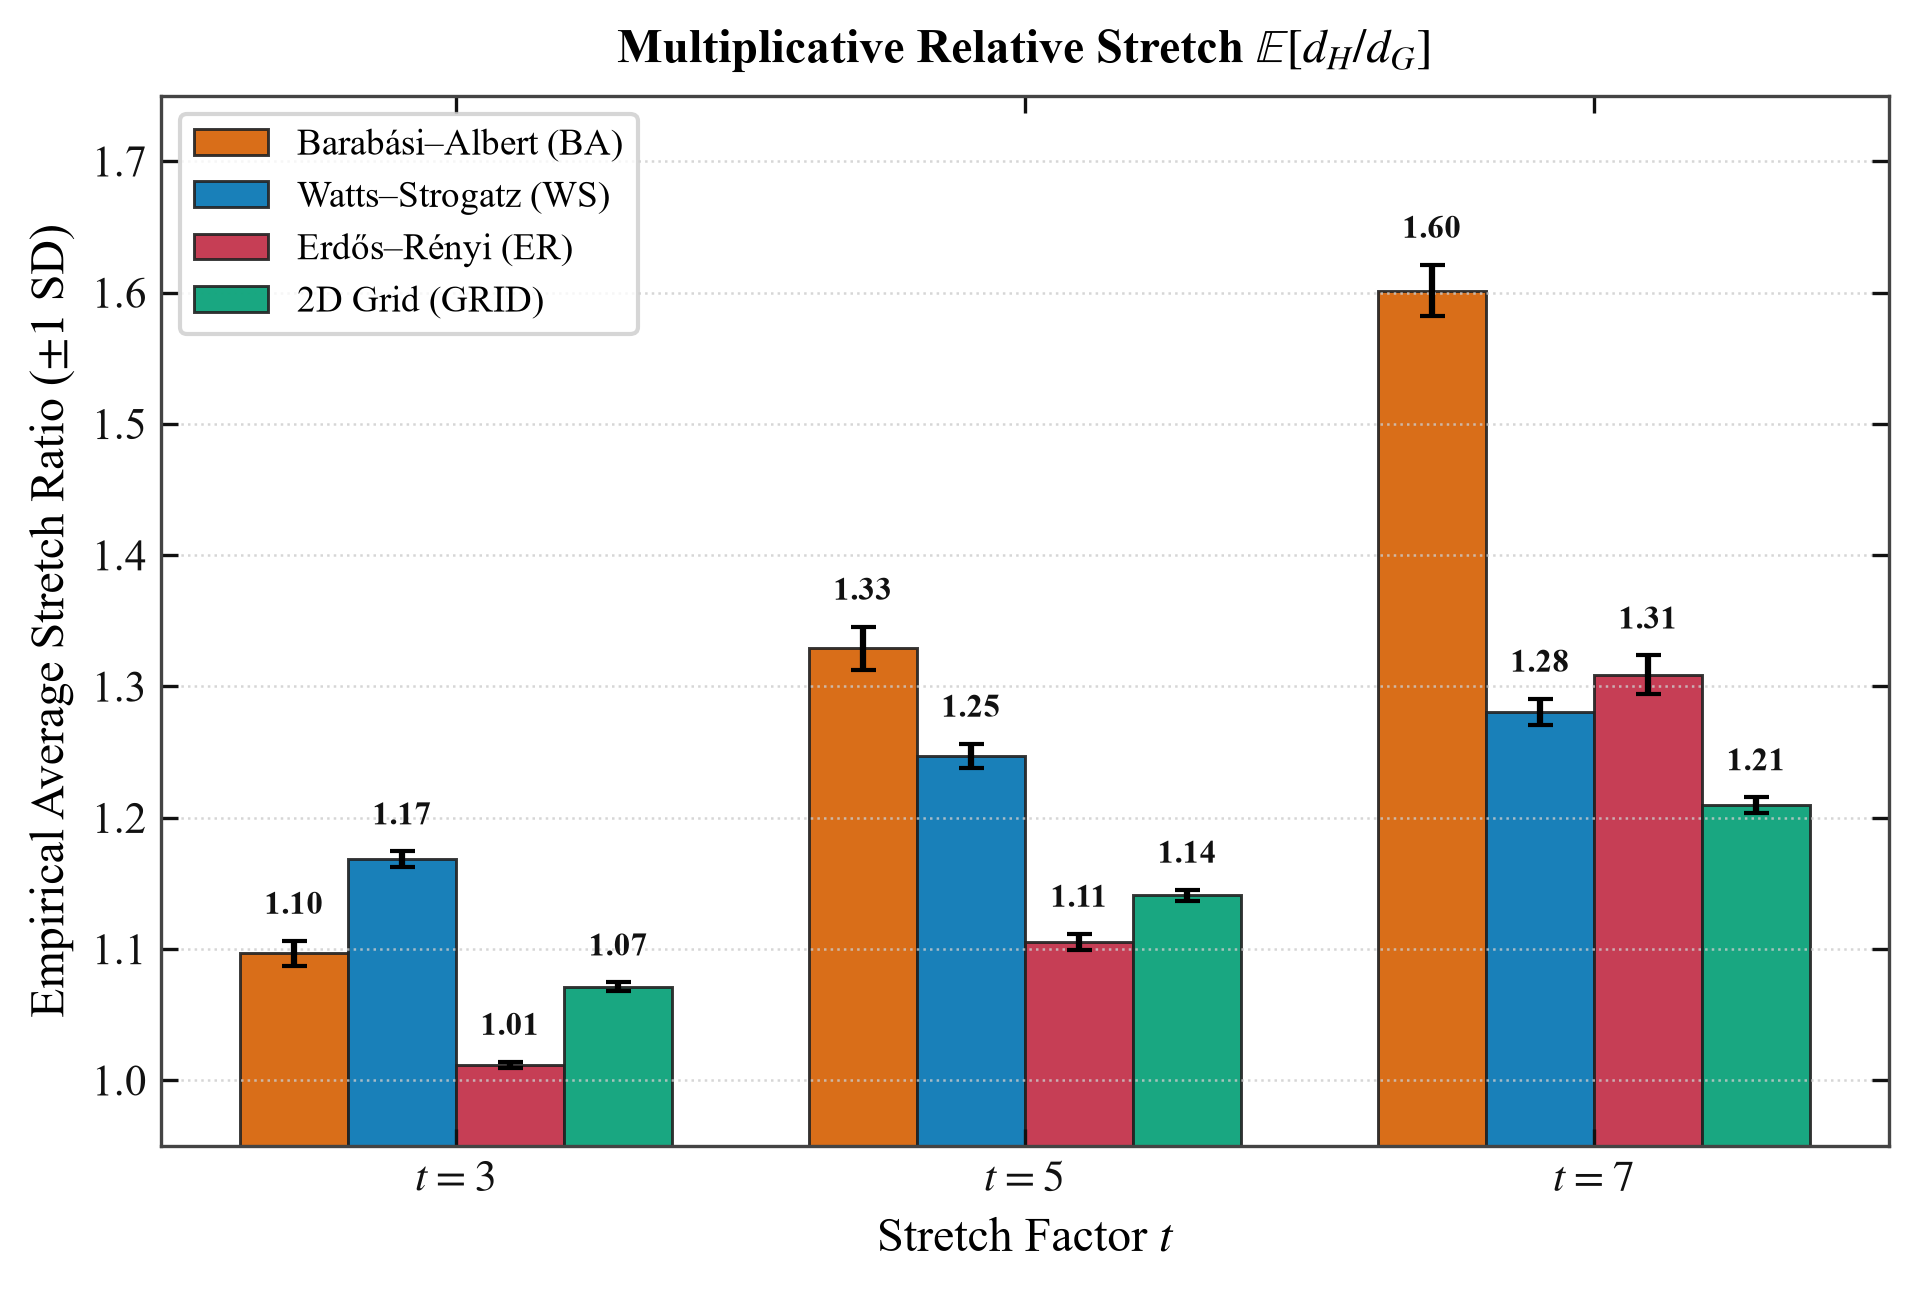
\includegraphics[width=\columnwidth]{figures/fig6_multiplicative.png}
    \caption{Mean multiplicative relative stretch across stretch factors $t \in \{3, 5, 7\}$. Scale-free hubs (BA) appear disadvantageous due to baseline path compression. Error bars represent $\pm 1$ SD across the $30$ independent graph-level means.}
    \label{fig:multiplicative_stretch}
\end{figure}

Under the standard multiplicative ratio metric (Fig.~\ref{fig:multiplicative_stretch}), BA exhibits significantly higher stretch than GRID across all stretch factors ($t=3$: $1.097$ vs.\ $1.071$; $t=5$: $1.329$ vs.\ $1.141$; $t=7$: $1.602$ vs.\ $1.210$). Consequently, the primary directional hypothesis test ($H_{a,2}: \mu_{\mathrm{BA}} < \mu_{\mathrm{GRID}}$) fails to reject $H_{0,2}$ across every stretch factor ($t=3$: directional Welch $p = 1.00$, Mann--Whitney $p = 1.00$; $t=7$: directional Welch $p = 1.00$, Mann--Whitney $p = 1.00$). Quantifying the observed difference in the opposite direction at $t=7$, the mean multiplicative stretch difference ($\mathrm{BA} - \mathrm{GRID}$) is $0.392$ ($95\%$ CI $[0.384, 0.400]$; two-sided Welch $t(34.4) = 104.06, p = 1.52 \times 10^{-44}$; Mann--Whitney $U = 900.0, p = 3.02 \times 10^{-11}$, Cohen's $d_{\mathrm{BA}-\mathrm{GRID}} = 26.87$). Under the primary multiplicative-stretch metric, BA exhibits significantly greater distortion than GRID. Therefore, $H_{0,2}$ is not rejected, and the directional alternative $H_{a,2}$ is not supported.

\begin{figure}[!t]
    \centering
    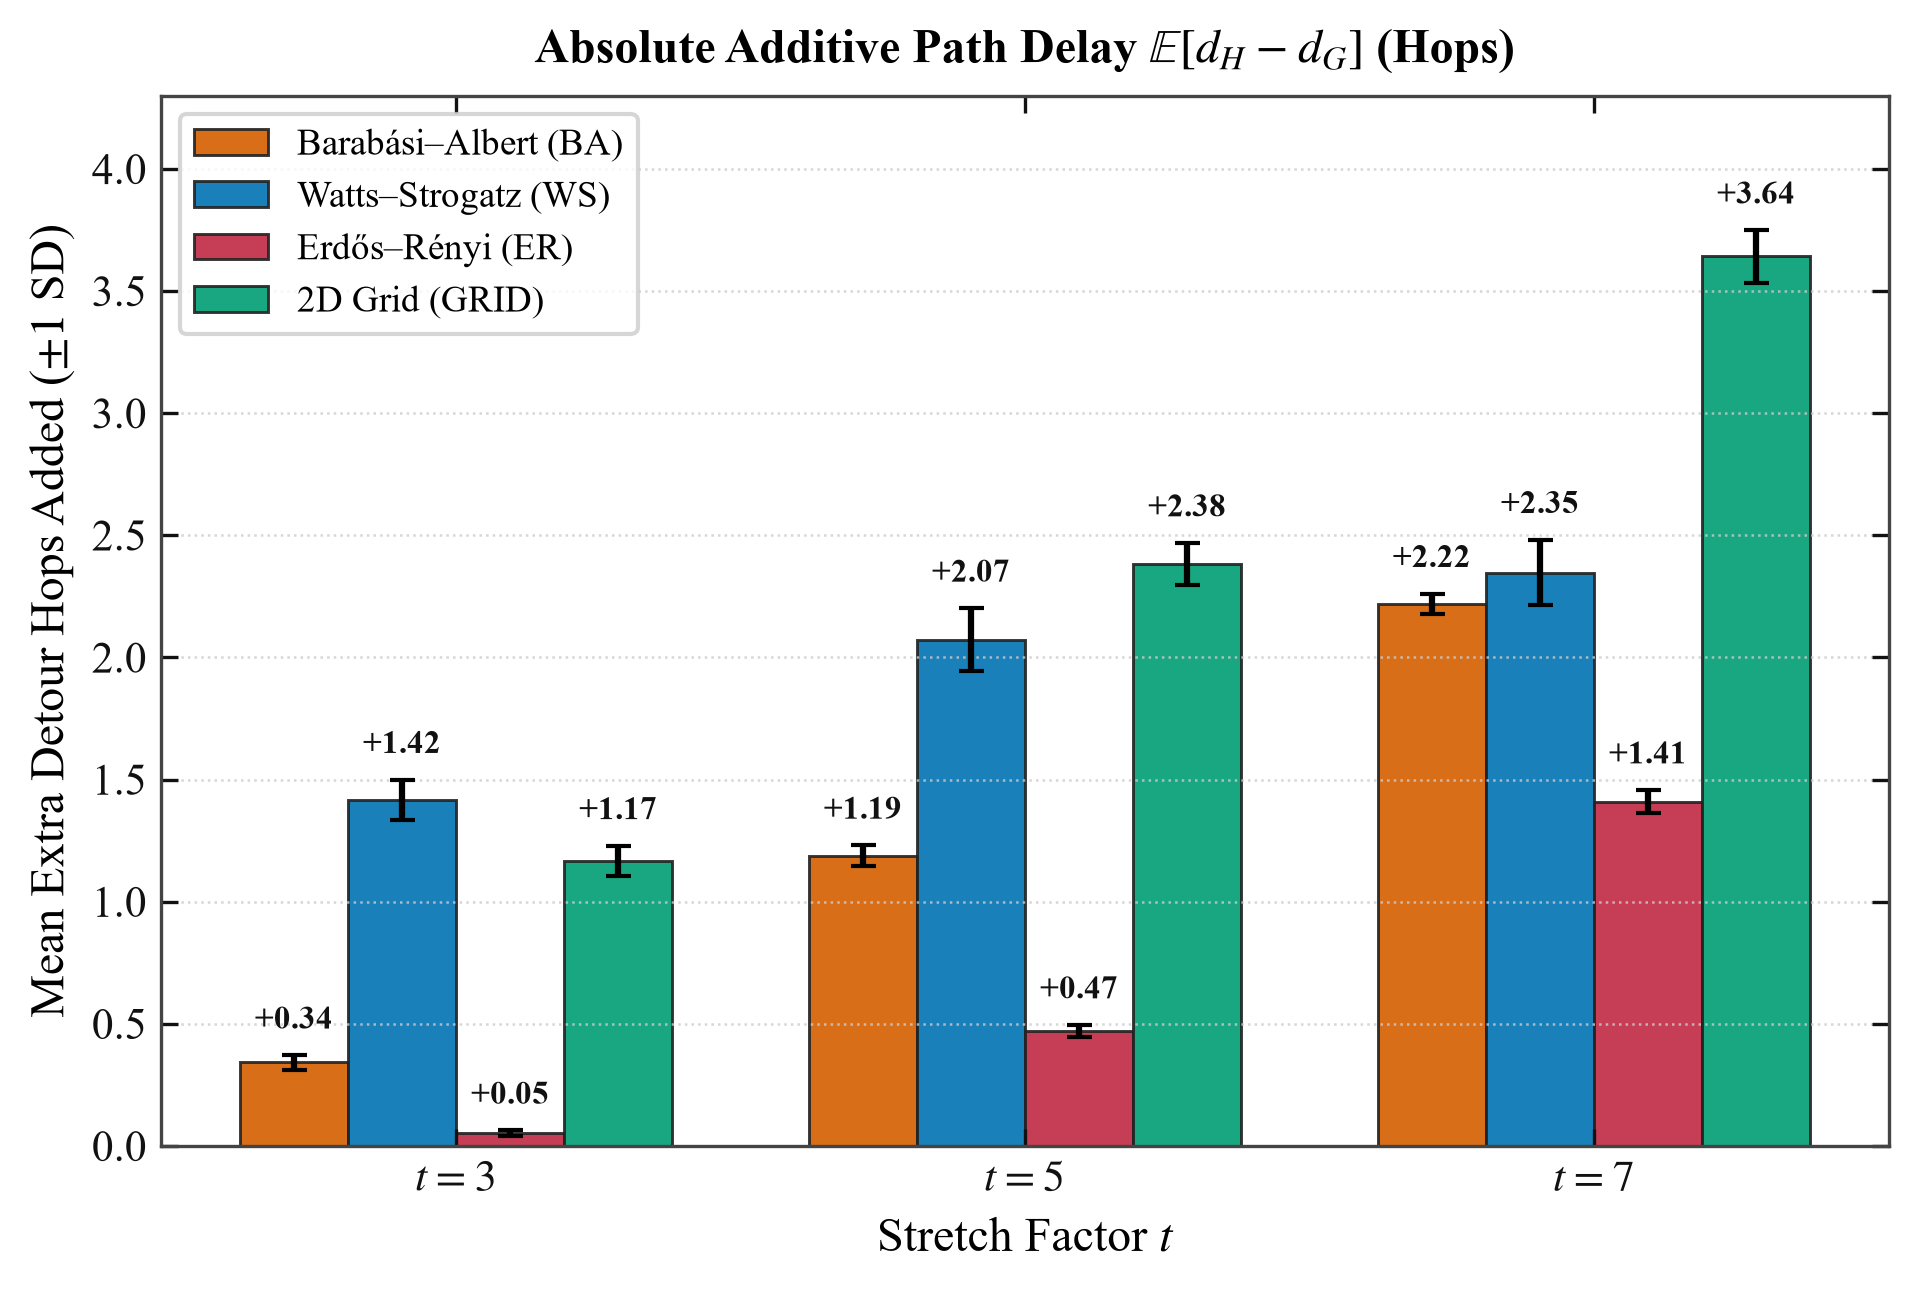
\includegraphics[width=\columnwidth]{figures/fig6_additive.png}
    \caption{Mean absolute additive path delay (extra detour hops added) across stretch factors $t \in \{3, 5, 7\}$. Planar grids incur significantly higher physical detours than scale-free hubs. Error bars represent $\pm 1$ SD across the $30$ independent graph-level means.}
    \label{fig:additive_delay}
\end{figure}

However, evaluating absolute additive path delay (Fig.~\ref{fig:additive_delay}) completely reverses this conclusion. Across all stretch factors, spanners on BA add far fewer physical detour hops than on GRID ($t=3$: $+0.34$ vs.\ $+1.17$ hops; $t=5$: $+1.19$ vs.\ $+2.38$ hops; $t=7$: $+2.22$ vs.\ $+3.64$ hops). At $t=7$, the mean physical detour gap ($\mathrm{GRID} - \mathrm{BA}$) is $1.42$ hops ($95\%$ CI $[1.38, 1.46]$ hops; directional Welch $t(37.1) = -68.01$ for $\mathrm{BA} - \mathrm{GRID}$, $p = 6.86 \times 10^{-41}$; Mann--Whitney $U = 0.0, p = 1.51 \times 10^{-11}$, Cohen's $d_{\mathrm{GRID}-\mathrm{BA}} = 17.56$).

This metric inversion demonstrates the \textit{baseline path-length dilution effect}: multiplicative stretch $d_H(u,v) / d_G(u,v) = 1 + \Delta d(u,v) / d_G(u,v)$ divides detour hops by the baseline path length $d_G$. Because BA has ultra-short baseline paths ($L = 4.06$), an additive detour of $+2.22$ hops produces a noticeable relative stretch ratio ($(4.06 + 2.22) / 4.06 \approx 1.55$, empirical mean $\bar{s} = 1.602$). Conversely, because GRID has very long baseline paths ($L = 21.70$), even a larger additive detour of $+3.64$ hops is diluted by the large denominator ($(21.70 + 3.64) / 21.70 \approx 1.17$, empirical mean $\bar{s} = 1.210$). These ratios of aggregate means are illustrative rather than exact estimates of empirical mean stretch, because the mean of pairwise distance ratios generally differs from the ratio of mean distances.

Whether scale-free networks exhibit lower path distortion depends on the evaluation metric: BA exhibits higher multiplicative stretch but lower mean additive hop delay ($+2.22$ hops at $t=7$) than GRID ($+3.64$ hops). The significantly lower additive delay observed in BA provides complementary evidence that scale-free networks exhibit smaller absolute detour lengths relative to planar grids. However, this secondary result does not overturn the primary multiplicative-stretch hypothesis test.

\subsection{Structural Correlates, Bound Slack, and Practicality (RQ3)}

\begin{figure*}[!t]
    \centering
    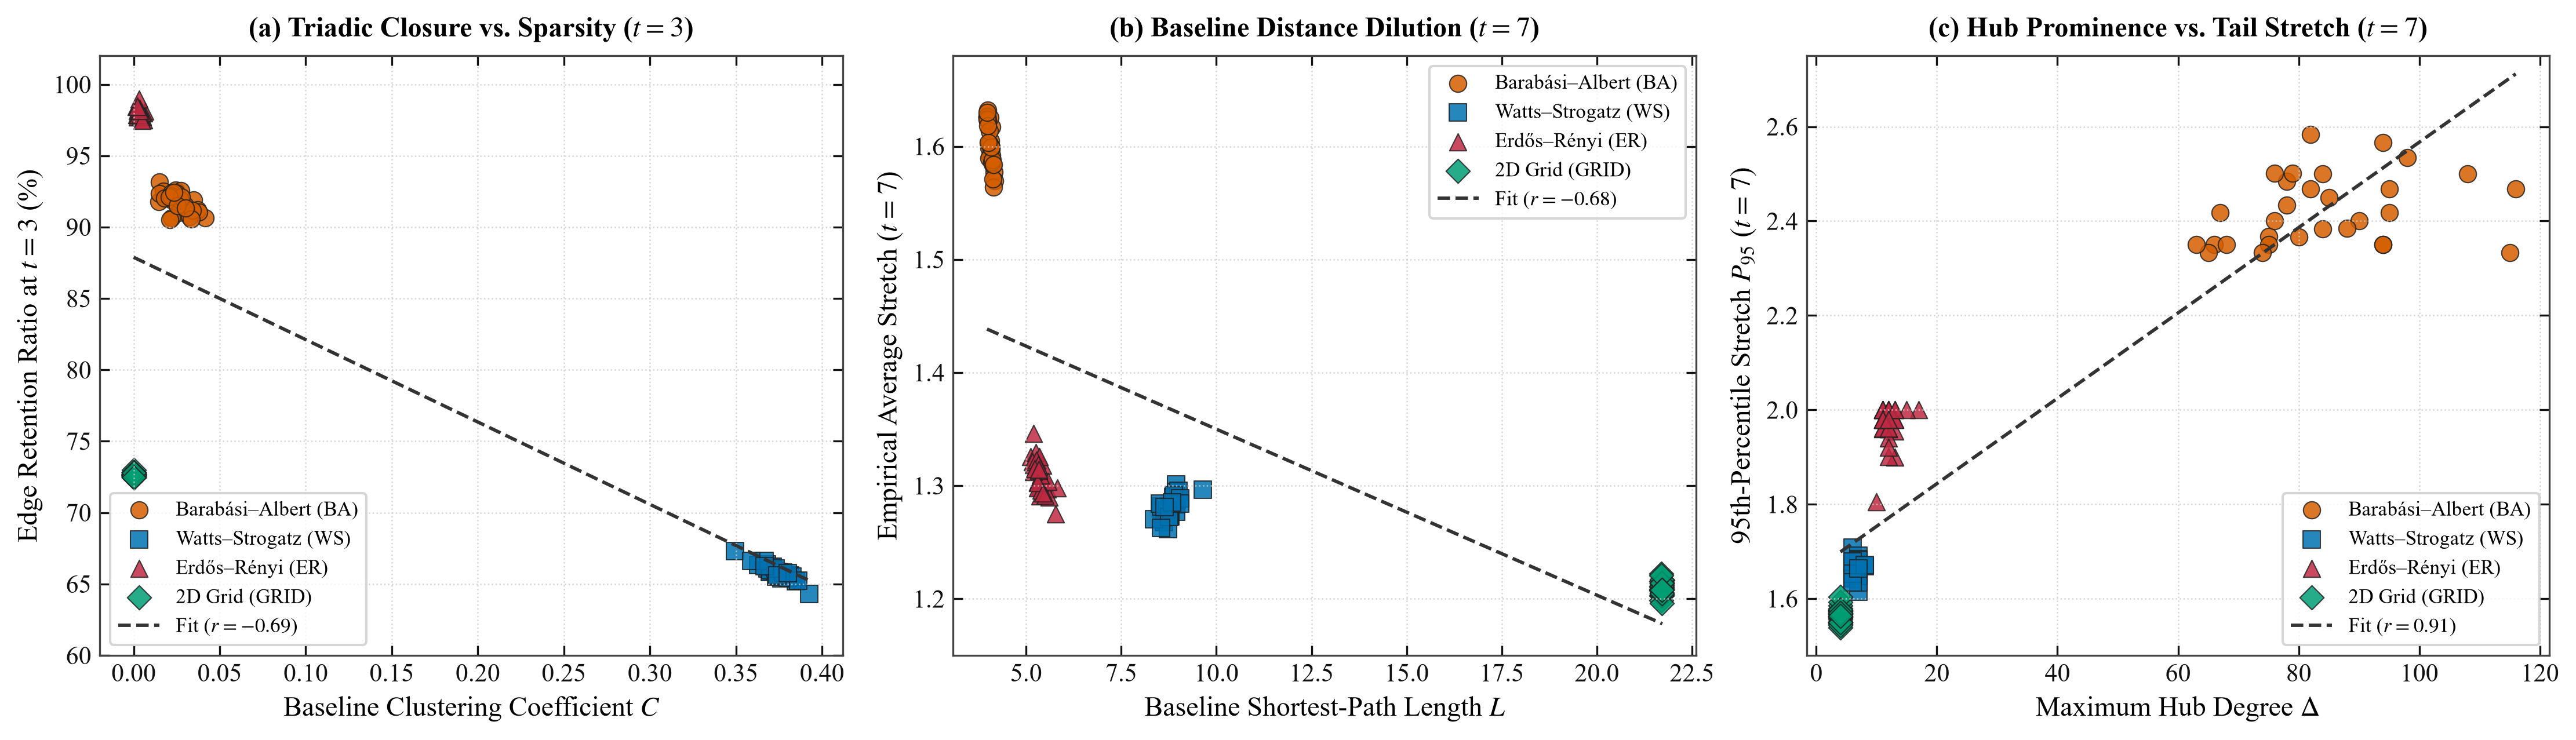
\includegraphics[width=0.98\textwidth]{figures/fig5_structural_mechanisms.png}
    \caption{Empirical associations between baseline structural metrics and spanner performance across all $120$ networks: (a) negative correlation between clustering coefficient $C$ and edge retention at $t=3$ ($r = -0.69$), (b) inverse correlation between baseline path length $L$ and average stretch at $t=7$ ($r = -0.68$), and (c) positive correlation between maximum hub degree $\Delta$ and 95th-percentile tail stretch at $t=7$ ($r = 0.91$).}
    \label{fig:mechanisms}
\end{figure*}

To evaluate RQ3 and test $H_{0,3}$, Fig.~\ref{fig:mechanisms} examines how baseline structural properties ($C, L, \Delta$) relate to spanner performance across all $120$ networks, alongside the bound slack and runtime metrics in Table~\ref{tab:main_results}. Because $C, L,$ and $\Delta$ cluster by generator family, these pooled Pearson correlations ($p < 10^{-17}$) primarily capture between-family structural regimes, rejecting $H_{0,3}$ in favor of $H_{a,3}$:

\begin{enumerate}
    \item \textit{Clustering ($C$) and Early Pruning [Fig.~\ref{fig:mechanisms}(a)]:} Baseline clustering correlates negatively with edge retention at $t=3$ ($r = -0.69$, $95\%$ CI $[-0.77, -0.58]$). Because the greedy algorithm discards an edge whenever $d_H(u, v) \le t$, every triangle ($3$-cycle) provides a potential $2$-hop bypass ($2 \le 3$) depending on edge-inspection order, enabling heavily clustered WS graphs to prune $34.1\%$ of their edges at $t=3$. Notice that GRID sits well below ER in Fig.~\ref{fig:mechanisms}(a) despite having $C = 0$: its $4$-cycles (unit squares) provide $3$-hop detours ($3 \le 3$) that allow $27.3\%$ pruning at $t=3$, whereas sparse ER graphs exhibit near-zero triangle clustering ($C = 0.0036 \pm 0.0013$; note that $C$ quantifies $3$-cycles rather than all longer short cycles).
    \item \textit{Baseline Path Length ($L$) and Stretch Dilution [Fig.~\ref{fig:mechanisms}(b)]:} Baseline path length correlates negatively with average stretch at $t=7$ ($r = -0.68$, $95\%$ CI $[-0.76, -0.57]$), consistent with the explanation that larger baseline path lengths buffer multiplicative stretch ratios as $L$ increases from BA ($L=4.06$) to GRID ($L=21.70$).
    \item \textit{Hub Prominence ($\Delta$) and Tail Stretch [Fig.~\ref{fig:mechanisms}(c)]:} Maximum degree $\Delta$ correlates strongly with 95th-percentile tail stretch at $t=7$ ($r = 0.91$, $95\%$ CI $[0.87, 0.94]$). While the topologies with lower observed maximum degrees (GRID, WS, ER) cluster below $P_{95} \le 2.00$, this association is consistent with paths in sparsified BA networks traversing high-degree hubs ($\Delta \in [63, 116]$), although vertex-level flow attribution was not directly measured.
    \item \textit{Sampled vs.\ Exact Bound Slack and Practicality (Table~\ref{tab:main_results}):} Across sampled vertex pairs ($M = 1,000$), observed route-level maximum stretch ($s_{\max}$) remains below the theoretical ceiling $t$ on average. Across all $120$ graphs at $t=7$, overall mean sampled bound slack is $2.34$ units ($95\%$ CI $[2.16, 2.52]$). Sampled bound slack is widest in WS ($3.59$ units) and GRID ($2.58$ units), whereas BA ($1.54$) and ER ($1.66$) approach closer to the limit $t$. Formal hypothesis testing confirms that these topological differences in sampled bound slack are statistically significant across all stretch limits ($F_W \ge 35.18, p < 10^{-12}$). In contrast, edge-level verification across original edges confirms that in $100\%$ of the $3,600$ constructions ($3,600/3,600$), at least one pruned edge attains an exact detour distance equal to $t$ ($s_{\max}^{\text{exact}} = t$, exact edge-level bound slack $= 0.00$). Similarly, Bounded-BFS runtime (Table~\ref{tab:main_results}) stays nearly flat from $t=3$ to $t=7$ on WS ($4.6 \to 6.9\text{ ms}$) and GRID ($7.2 \to 10.1\text{ ms}$) because local searches remain spatially bounded, but rises to $86.4\text{ ms}$ on BA ($12.5\times$ slower than WS), consistent with depth-$7$ breadth-first searches expanding rapidly through high-degree hubs. Finally, the condition-level within-graph standard deviation of edge retention across the $10$ random edge permutations remains below $0.65\%$ across all topological families ($0.05\%$ to $0.62\%$; max $1.02\%$ on any individual instance), confirming that unweighted greedy spanner sparsity is highly stable against random tie-breaking order.
\end{enumerate}

\subsection{Potential Architectural Implications and Practical Guidelines}

Synthesizing these empirical findings yields three potential design considerations for network architects:

\begin{enumerate}
    \item \textit{Leverage Local Clustering for Low-Stretch Sparsification:} In our evaluated small-world WS networks ($C = 0.3735$), greedy spanners achieve $34.1\%$ edge pruning immediately at $t=3$ with small average hop stretch ($\bar{s} = 1.168$). Operators in similarly clustered overlay or mesh domains could explore greedy spanners at low $t$ as a candidate mechanism for reducing link counts and routing-table size, subject to routing-protocol and link-capacity evaluation.
    \item \textit{Account for Hub Prominence in Scale-Free Backbones:} In preferential attachment topologies (such as Internet autonomous systems or airline route maps), operators should not rely on multiplicative stretch ratios alone to assess path quality, as baseline path compression yields elevated stretch numbers relative to additive hop delay. More critically, high-$t$ sparsification in BA networks is associated with elevated 95th-percentile path stretch ($P_{95} = 2.42$). Potential implications for tail latency and hub congestion require further traffic-level evaluation.
    \item \textit{Consider the Stretch--Sparsity Trade-Off in Planar Infrastructures:} For planar topologies (such as transportation lattices or VLSI layout grids), greedy spanners provide steady, predictable edge pruning ($39.2\%$ pruned at $t=7$) with the lowest average stretch ($\bar{s} = 1.21$) and generous sampled bound slack ($2.58$ units, while noting that worst-case edge-level stretch still attains $t$).
\end{enumerate}

% ============================================================================
% SECTION VII: THREATS TO VALIDITY
% ============================================================================
\section{Threats to Validity}

\subsection{Internal Validity}
Although baseline density was targeted at $\bar{d} \approx 4.0$, minor generator variations exist: perturbed grids have slightly lower density ($\bar{d} = 3.79$) due to boundary vertices and $2\%$ random edge removal, whereas sparse ER graphs required minimal chain-repair augmentation ($c - 1 = 18.8 \pm 3.1$ bridge edges, $< 1\%$ of $|E_G|$) to guarantee connectivity. While mandatory bridge retention ($4.97\%$ of $|E_G|$ in ER including natural leaves) cannot alone explain ER's near-total edge retention, given that over $97.9\%$ of its non-bridge cyclic edges also resisted pruning at $t = 3$, the repair procedure remains a minor structural artifact that must be accounted for when interpreting retention. To mitigate deterministic tie-breaking bias in unweighted graphs, we evaluated $10$ uniform random edge permutations per instance at each $t$, confirming that within-graph retention standard deviation averaged $0.30\%$ overall ($0.05\%\text{--}0.62\%$ across conditions). Finally, reported runtimes ($4.6\text{--}86.4\text{ ms}$) reflect relative bounded-BFS traversal effort across topologies rather than compiled production benchmarks.

\subsection{External Validity}
Our study evaluates four synthetic canonical generators (BA, WS, ER, and perturbed GRID) representing distinct topological regimes with contrasting profiles of ($\Delta$, $C$, and $L$), rather than independently manipulating single structural invariants in isolation. Real-world communication and infrastructure networks often exhibit hybrid topologies combining scale-free degree distributions with modular clustering. Additionally, evaluations were restricted to unweighted, undirected networks at a fixed scale ($N = 1,000$, $\bar{d} \approx 3.8\text{--}4.0$, $t \in \{3, 5, 7\}$). While this scale exposes structural girth bottlenecks and finite-diameter baseline effects ($D = 7.20$ in BA), massive networks ($N \ge 10^6$), dense regimes ($\bar{d} \gg \log N$), or weighted graphs with continuous edge-weight tie-breaking may follow different pruning trajectories.

\subsection{Construct Validity}
To maintain computational tractability across $3,600$ spanner constructions, stretch metrics ($\bar{s}$, $P_{95}$, and $s_{\max}$) were evaluated over $M = 1,000$ unordered vertex pairs sampled uniformly without replacement from all $\binom{1,000}{2} = 499,500$ possible pairs. Caching and reusing the same pair sets across stretch factors and permutations controls cross-condition sampling variation, though it does not eliminate sampling uncertainty. Because the sampled maximum stretch $s_{\max}$ is a lower bound on the true network-wide maximum stretch, the empirical bound slack ($t - s_{\max}$) may overestimate the true worst-case slack across the full graph. Although sampled maximum stretch may underestimate the true global maximum, the additional edge-level verification establishes exact maximum stretch independently of vertex-pair sampling. Furthermore, because multiplicative stretch ($d_H / d_G$) scales inversely with baseline distance $d_G$ (path-length dilution), relying on it alone misrepresents physical hop detours; evaluating additive hop delay ($d_H - d_G$) ensures a balanced assessment of path distortion.

\subsection{Statistical Conclusion Validity}
To prevent pseudoreplication, the $10$ edge permutations per instance were averaged into a single graph-level mean prior to hypothesis testing, restricting all tests to $n = 30$ independent instances per topology. Significant heteroscedasticity across topologies (Levene's test, $W \ge 13.11, p < 2.0 \times 10^{-7}$) was addressed by pairing Welch's heteroscedastic ANOVA \cite{ref27} and $t$-tests with non-parametric Kruskal--Wallis and Mann--Whitney $U$ tests. To control Type I error across multiple comparisons without selection bias, Holm--Bonferroni step-down and Benjamini--Hochberg False Discovery Rate (FDR) adjustments were applied \textit{a priori} across all $12$ RQ2 Welch pairwise tests (the $9$ supported comparisons remain at $p_{\mathrm{adj}} \le 1.67 \times 10^{-15}$, whereas the $3$ directional tests for $H_{a,2}: \mu_{\mathrm{BA}} < \mu_{\mathrm{GRID}}$ on $\bar{s}$ remain non-significant with $p_{\mathrm{adj}} = 1.00$) and across the complete study-wide family of all $45$ inferential hypothesis tests ($12$ in RQ1, $24$ in RQ2 including all $6$ non-significant directional multiplicative tests with $p_{\mathrm{adj}} = 1.00$, and $9$ in RQ3). Under this full $45$-test correction, all $39$ supported findings remained overwhelmingly statistically significant: all $21$ supported parametric tests satisfied $p_{\mathrm{adj}} < 3 \times 10^{-12}$ (Holm max $= 2.87 \times 10^{-12}$, FDR max $= 2.62 \times 10^{-13}$) and all $18$ supported non-parametric and rank-correlation tests satisfied $p_{\mathrm{adj}} < 4 \times 10^{-5}$ (Holm max $= 3.06 \times 10^{-5}$, FDR max $= 5.05 \times 10^{-6}$). Finally, the pooled correlations ($N = 120$) in RQ3 capture macroscopic associations across generator families rather than within-family causal mechanisms.

% ============================================================================
% SECTION VIII: CONCLUSION AND FUTURE WORK
% ============================================================================
\section{Conclusion and Future Work}

This paper presented an empirical evaluation of the classical greedy $t$-spanner algorithm across four canonical graph topologies (Barab\'{a}si--Albert, Watts--Strogatz, Erd\H{o}s--R\'{e}nyi, and perturbed 2D Grids) under a fixed vertex count ($N = 1,000$) and closely matched baseline density ($\bar{d} \approx 3.79\text{--}4.04$). Across $3,600$ factorial spanner constructions, our findings demonstrate that when baseline density is held approximately constant, spanner pruning efficiency differs sharply across topologies and is strongly associated with differences in local cycle structure and clustering across topological families. High clustering ($C = 0.374$) in Watts--Strogatz networks provides immediate triangle-based alternate paths that allow the greedy algorithm to prune $34.1\%$ of edges at $t = 3$ and $40.4\%$ at $t = 7$. Conversely, locally tree-like Erd\H{o}s--R\'{e}nyi graphs exhibiting near-zero triangle clustering ($C \approx 0.004$) retain $98.0\%$ of edges at $t = 3$ and continue to retain $75.4\%$ even at $t = 7$, yielding the lowest edge reduction among all evaluated topologies.

Furthermore, we resolved the apparent conflict between multiplicative stretch and additive hop distortion through the baseline path-length dilution effect. Due to the inverse dependence of excess multiplicative stretch on baseline distance for a fixed additive detour, planar grids with long paths ($L \approx 21.7$) exhibit low multiplicative stretch ($\bar{s} \le 1.21$) yet incur larger mean additive hop detours ($+3.64$ hops at $t = 7$). Combining additive hop delay with multiplicative stretch showed that scale-free networks with short diameters incur lower mean additive detour hops ($+2.22$ hops at $t = 7$) while exhibiting elevated 95th-percentile tail stretch ($P_{95} = 2.42$). Although empirical average stretch remained substantially below the theoretical limit, exact maximum stretch attained $t$ in all $3,600$ constructions. At $t=7$, the mean sampled bound slack was $2.34$ units ($95\%$ CI $[2.16, 2.52]$), whereas exact bound slack was zero. This distinction highlights the difference between typical sampled path distortion and worst-case stretch guarantees.

These results give architectural insights suggesting that greedy spanners can be promising candidates for the development of clustered overlay networks but may offer limited edge sparsification in sparse and tree-like structures without any structural pre-processing that warrant empirical validation in real-world systems. In future work, we intend to apply this benchmark to weighted infrastructure graphs where edges have deterministic order determined by the weight of links, study hybrid topologies with the scale-free degree distribution and community clustering, and consider maintenance of dynamic and fault-tolerant spanners \cite{ref26}.

\section*{Acknowledgment}
The authors thank the College of Information and Computer Science (ICS) at King Fahd University of Petroleum and Minerals (KFUPM) for supporting this research. Generative AI tools were utilized for language editing, code and statistical verification assistance, literature auditing, and LaTeX typesetting; the authors independently verified all implementations, empirical data, and scientific conclusions, which remain the sole work and responsibility of the authors.

% ============================================================================
% REFERENCES
% ============================================================================
\begin{thebibliography}{27}

\bibitem{ref1}
Y. Chen \textit{et al.},
``Demystifying graph sparsification algorithms in graph properties preservation,''
\textit{Proc. VLDB Endow.},
vol. 17, no. 3, pp. 427--440, 2023,
doi: 10.14778/3632093.3632106.

\bibitem{ref2}
I. Alth\"{o}fer, G. Das, D. Dobkin, D. Joseph, and J. Soares,
``On sparse spanners of weighted graphs,''
\textit{Discrete \& Computational Geometry},
vol. 9, no. 1, pp. 81--100, 1993,
doi: 10.1007/BF02189308.

\bibitem{ref3}
D. Peleg and A. A. Sch\"{a}ffer,
``Graph spanners,''
\textit{Journal of Graph Theory},
vol. 13, no. 1, pp. 99--116, 1989,
doi: 10.1002/jgt.3190130114.

\bibitem{ref4}
R. Ahmed \textit{et al.},
``Graph spanners: A tutorial review,''
\textit{Computer Science Review},
vol. 37, Art. no. 100253, 2020,
doi: 10.1016/j.cosrev.2020.100253.

\bibitem{ref5}
A. Filtser and S. Solomon,
``The greedy spanner is existentially optimal,''
\textit{SIAM Journal on Computing},
vol. 49, no. 2, pp. 429--447, 2020,
doi: 10.1137/18M1210678.

\bibitem{ref6}
F. B\"{o}kler, M. Chimani, and H. Jasper,
``General multiplicative spanners in practice,''
in \textit{Proc. 24th Int. Symp. Experimental Algorithms (SEA)},
Schloss Dagstuhl--Leibniz-Zentrum f\"{u}r Informatik, 2026, pp. 8:1--8:21,
doi: 10.4230/LIPIcs.SEA.2026.8.

\bibitem{ref7}
H. Le, S. Solomon, C. Than, C. D. T\'{o}th, and T. Zhang,
``Towards instance-optimal Euclidean spanners,''
in \textit{Proc. IEEE 65th Annu. Symp. Foundations of Computer Science (FOCS)},
2024, pp. 1579--1609,
doi: 10.1109/FOCS61266.2024.00099.

\bibitem{ref8}
M. Farshi and J. Gudmundsson,
``Experimental study of geometric $t$-spanners,''
in \textit{Proc. 13th Annu. European Symp. Algorithms (ESA)},
Berlin, Heidelberg: Springer, 2005, pp. 556--567,
doi: 10.1007/11561071\_50.

\bibitem{ref9}
M. Farshi and J. Gudmundsson,
``Experimental study of geometric $t$-spanners,''
\textit{ACM Journal of Experimental Algorithmics (JEA)},
vol. 14, Art. no. 1.3, pp. 1.3:1--1.3:29, 2009,
doi: 10.1145/1498698.1564499.

\bibitem{ref10}
R. Ahmed, G. Bodwin, F. D. Sahneh, K. Hamm, S. Kobourov, and R. Spence,
``Multi-level weighted additive spanners,''
in \textit{Proc. 19th Int. Symp. Experimental Algorithms (SEA)},
2021, pp. 16:1--16:23,
doi: 10.4230/LIPIcs.SEA.2021.16.

\bibitem{ref11}
L. Cunha, E. Marciano, A. Moraes, L. Santiago, and C. Santos,
``New parallelism and heuristic approaches for generating tree $t$-spanners in graphs,''
\textit{Concurrency and Computation: Practice and Experience},
vol. 36, no. 15, Art. no. e8106, 2024,
doi: 10.1002/cpe.8106.

\bibitem{ref12}
F. Couto, L. F. I. Cunha, D. Juventude, and L. Santiago,
``Strategies for generating tree spanners: Algorithms, heuristics and optimal graph classes,''
\textit{Information Processing Letters},
vol. 177, Art. no. 106265, 2022,
doi: 10.1016/j.ipl.2022.106265.

\bibitem{ref13}
A.-L. Barab\'{a}si and R. Albert,
``Emergence of scaling in random networks,''
\textit{Science},
vol. 286, no. 5439, pp. 509--512, 1999,
doi: 10.1126/science.286.5439.509.

\bibitem{ref14}
D. J. Watts and S. H. Strogatz,
``Collective dynamics of `small-world' networks,''
\textit{Nature},
vol. 393, no. 6684, pp. 440--442, 1998,
doi: 10.1038/30918.

\bibitem{ref15}
P. Erd\H{o}s and A. R\'{e}nyi,
``On the evolution of random graphs,''
\textit{Publ. Math. Inst. Hung. Acad. Sci.},
vol. 5, no. 1, pp. 17--61, 1960.

\bibitem{ref16}
A. M. Farley, A. Proskurowski, D. Zappala, and K. Windisch,
``Spanners and message distribution in networks,''
\textit{Discrete Applied Mathematics},
vol. 137, no. 2, pp. 159--171, 2004,
doi: 10.1016/S0166-218X(03)00259-2.

\bibitem{ref17}
G. Bodwin,
``An alternate proof of near-optimal light spanners,''
\textit{TheoretiCS},
vol. 4, Art. no. 2, 2025,
doi: 10.46298/theoretics.25.2.

\bibitem{ref18}
H. Le and S. Solomon,
``A unified framework for light spanners,''
in \textit{Proc. 55th Annu. ACM Symp. Theory of Computing (STOC)},
2023, pp. 295--308,
doi: 10.1145/3564246.3585185.

\bibitem{ref19}
G. Bodwin and J. Flics,
``A lower bound for light spanners in general graphs,''
in \textit{Proc. Annu. ACM-SIAM Symp. Discrete Algorithms (SODA)},
SIAM, 2025, pp. 4327--4337,
doi: 10.1137/1.9781611978322.146.

\bibitem{ref20}
N. K\={o}shima, T. Rieder, S. Basu, T. Eden, and O. Ben-Eliezer,
``Density-accuracy tradeoffs in real-world graph spanners,''
presented at the \textit{SIAM Conf. Applied and Computational Discrete Algorithms (ACDA)},
2025, extended abstract.

\bibitem{ref21}
M. Chimani and F. Stutzenstein,
``Spanner approximations in practice,''
in \textit{Proc. 30th Annu. European Symp. Algorithms (ESA)},
2022, pp. 37:1--37:15,
doi: 10.4230/LIPIcs.ESA.2022.37.

\bibitem{ref22}
A. Ghosh,
``Constructing doppelg\"{a}ngers of greedy geometric spanners in practice,''
in \textit{Proc. 42nd Int. Symp. Computational Geometry (SoCG)},
Schloss Dagstuhl--Leibniz-Zentrum f\"{u}r Informatik, 2026, pp. 53:1--53:21,
doi: 10.4230/LIPIcs.SoCG.2026.53.

\bibitem{ref23}
B. Haeupler, D. E. Hershkowitz, and Z. Tan,
``Parallel greedy spanners,''
\textit{arXiv preprint arXiv:2304.08892}, 2023.

\bibitem{ref24}
L. Breslau \textit{et al.},
``Advances in network simulation,''
\textit{IEEE Computer},
vol. 33, no. 5, pp. 59--67, 2000,
doi: 10.1109/2.841785.

\bibitem{ref25}
M. Thorup and U. Zwick,
``Compact routing schemes,''
in \textit{Proc. 13th Annu. ACM Symp. Parallel Algorithms and Architectures (SPAA)},
2001, pp. 1--10,
doi: 10.1145/378580.378581.

\bibitem{ref26}
G. Bodwin, M. Dinitz, A. Koranteng, and L. Wang,
``Light edge fault tolerant graph spanners,''
in \textit{Proc. 52nd Int. Colloquium Automata, Languages, and Programming (ICALP)},
2025, pp. 32:1--32:20,
doi: 10.4230/LIPIcs.ICALP.2025.32.

\bibitem{ref27}
M. Delacre, C. Leys, Y. L. Mora, and D. Lakens,
``Taking parametric assumptions seriously: Arguments for the use of Welch's $F$-test instead of the classical $F$-test in one-way ANOVA,''
\textit{International Review of Social Psychology},
vol. 32, no. 1, Art. no. 13, 2019,
doi: 10.5334/irsp.198.

\end{thebibliography}   

\end{document}